\documentclass{beamer}

% xcolor and define colors -------------------------
\usepackage{xcolor}

% https://www.viget.com/articles/color-contrast/
\definecolor{purple}{HTML}{5601A4}
\definecolor{navy}{HTML}{0D3D56}
\definecolor{ruby}{HTML}{9a2515}
\definecolor{alice}{HTML}{107895}
\definecolor{daisy}{HTML}{EBC944}
\definecolor{coral}{HTML}{F26D21}
\definecolor{kelly}{HTML}{829356}
\definecolor{cranberry}{HTML}{E64173}
\definecolor{jet}{HTML}{131516}
\definecolor{asher}{HTML}{555F61}
\definecolor{slate}{HTML}{314F4F}

% Mixtape Sessions
\definecolor{picton-blue}{HTML}{00b7ff}
\definecolor{violet-red}{HTML}{ff3881}
\definecolor{sun}{HTML}{ffaf18}
\definecolor{electric-violet}{HTML}{871EFF}

\newcommand\pictonBlue[1]{{\color{picton-blue}#1}}
\newcommand\sun[1]{{\color{sun}#1}}
\newcommand\electricViolet[1]{{\color{electric-violet}#1}}
\newcommand\violetRed[1]{{\color{violet-red}#1}}

\newcommand\bgPictonBlue[1]{{\colorbox{picton-blue!20!white}{#1}}}
\newcommand\bgSun[1]{{\colorbox{sun!20!white}{#1}}}
\newcommand\bgElectricViolet[1]{{\colorbox{electric-violet!20!white}{#1}}}
\newcommand\bgVioletRed[1]{{\colorbox{violet-red!20!white}{#1}}}

\def\code#1{\texttt{#1}}

% Main theme colors
\definecolor{accent}{HTML}{00b7ff}
\definecolor{accent2}{HTML}{871EFF}
\definecolor{gray100}{HTML}{f3f4f6}
\definecolor{gray800}{HTML}{1F292D}


% Beamer Options -------------------------------------

% Background
\setbeamercolor{background canvas}{bg = white}

% Change text margins
\setbeamersize{text margin left = 15pt, text margin right = 15pt} 

% \alert
\setbeamercolor{alerted text}{fg = accent2}

% Frame title
\setbeamercolor{frametitle}{bg = white, fg = jet}
\setbeamercolor{framesubtitle}{bg = white, fg = accent}
\setbeamerfont{framesubtitle}{size = \small, shape = \itshape}

% Block
\setbeamercolor{block title}{fg = white, bg = accent2}
\setbeamercolor{block body}{fg = gray800, bg = gray100}

% Title page
\setbeamercolor{title}{fg = gray800}
\setbeamercolor{subtitle}{fg = accent}

%% Custom \maketitle and \titlepage
\setbeamertemplate{title page}
{
    %\begin{centering}
        \vspace{20mm}
        {\Large \usebeamerfont{title}\usebeamercolor[fg]{title}\inserttitle}\\
        {\large \itshape \usebeamerfont{subtitle}\usebeamercolor[fg]{subtitle}\insertsubtitle}\\ \vspace{10mm}
        {\insertauthor}\\
        {\color{asher}\small{\insertdate}}\\
    %\end{centering}
}

% Table of Contents
\setbeamercolor{section in toc}{fg = accent!70!jet}
\setbeamercolor{subsection in toc}{fg = jet}

% Button 
\setbeamercolor{button}{bg = accent}

% Remove navigation symbols
\setbeamertemplate{navigation symbols}{}

% Table and Figure captions
\setbeamercolor{caption}{fg=jet!70!white}
\setbeamercolor{caption name}{fg=jet}
\setbeamerfont{caption name}{shape = \itshape}

% Bullet points

%% Fix spacing between items
\let\olditemize=\itemize 
\let\endolditemize=\enditemize 
\renewenvironment{itemize}{\vspace{0.25em}\olditemize \itemsep0.25em}{\endolditemize}

%% Fix left-margins
\settowidth{\leftmargini}{\usebeamertemplate{itemize item}}
\addtolength{\leftmargini}{\labelsep}

%% enumerate item color
\setbeamercolor{enumerate item}{fg = accent}
\setbeamerfont{enumerate item}{size = \small}
\setbeamertemplate{enumerate item}{\insertenumlabel.}

%% itemize
\setbeamercolor{itemize item}{fg = accent!70!white}
\setbeamerfont{itemize item}{size = \small}
\setbeamertemplate{itemize item}[circle]

%% right arrow for subitems
\setbeamercolor{itemize subitem}{fg = accent!60!white}
\setbeamerfont{itemize subitem}{size = \small}
\setbeamertemplate{itemize subitem}{$\rightarrow$}

\setbeamertemplate{itemize subsubitem}[square]
\setbeamercolor{itemize subsubitem}{fg = jet}
\setbeamerfont{itemize subsubitem}{size = \small}








% Links ----------------------------------------------

\usepackage{hyperref}
\hypersetup{
  colorlinks = true,
  linkcolor = accent2,
  filecolor = accent2,
  urlcolor = accent2,
  citecolor = accent2,
}


% Line spacing --------------------------------------
\usepackage{setspace}
\setstretch{1.35}


% \begin{columns} -----------------------------------
\usepackage{multicol}


% Fonts ---------------------------------------------
% Beamer Option to use custom fonts
\usefonttheme{professionalfonts}

% \usepackage[utopia, smallerops, varg]{newtxmath}
% \usepackage{utopia}
\usepackage[sfdefault,light]{roboto}

% Small adjustments to text kerning
\usepackage{microtype}



% Remove annoying over-full box warnings -----------
\vfuzz2pt 
\hfuzz2pt


% Table of Contents with Sections
\setbeamerfont{myTOC}{series=\bfseries, size=\Large}
\AtBeginSection[]{
        \frame{
            \frametitle{Roadmap}
            \tableofcontents[current]   
        }
    }


% Tables -------------------------------------------
% Tables too big
% \begin{adjustbox}{width = 1.2\textwidth, center}
\usepackage{adjustbox}
\usepackage{array}
\usepackage{threeparttable, booktabs, adjustbox}
    
% Fix \input with tables
% \input fails when \\ is at end of external .tex file
\makeatletter
\let\input\@@input
\makeatother

% Tables too narrow
% \begin{tabularx}{\linewidth}{cols}
% col-types: X - center, L - left, R -right
% Relative scale: >{\hsize=.8\hsize}X/L/R
\usepackage{tabularx}
\newcolumntype{L}{>{\raggedright\arraybackslash}X}
\newcolumntype{R}{>{\raggedleft\arraybackslash}X}
\newcolumntype{C}{>{\centering\arraybackslash}X}

% Figures

% \imageframe{img_name} -----------------------------
% from https://github.com/mattjetwell/cousteau
\newcommand{\imageframe}[1]{%
    \begin{frame}[plain]
        \begin{tikzpicture}[remember picture, overlay]
            \node[at = (current page.center), xshift = 0cm] (cover) {%
                \includegraphics[keepaspectratio, width=\paperwidth, height=\paperheight]{#1}
            };
        \end{tikzpicture}
    \end{frame}%
}

% subfigures
\usepackage{subfigure}


% Highlight slide -----------------------------------
% \begin{transitionframe} Text \end{transitionframe}
% from paulgp's beamer tips
\newenvironment{transitionframe}{
    \setbeamercolor{background canvas}{bg=accent!40!black}
    \begin{frame}\color{accent!10!white}\LARGE\centering
}{
    \end{frame}
}


% Table Highlighting --------------------------------
% Create top-left and bottom-right markets in tabular cells with a unique matching id and these commands will outline those cells
\usepackage[beamer,customcolors]{hf-tikz}
\usetikzlibrary{calc}
\usetikzlibrary{fit,shapes.misc}

% To set the hypothesis highlighting boxes red.
\newcommand\marktopleft[1]{%
    \tikz[overlay,remember picture] 
        \node (marker-#1-a) at (0,1.5ex) {};%
}
\newcommand\markbottomright[1]{%
    \tikz[overlay,remember picture] 
        \node (marker-#1-b) at (0,0) {};%
    \tikz[accent!80!jet, ultra thick, overlay, remember picture, inner sep=4pt]
        \node[draw, rectangle, fit=(marker-#1-a.center) (marker-#1-b.center)] {};%
}


% DAGS ----------------------------------------------
\usepackage{tikz}
\usetikzlibrary{shapes,decorations,arrows,calc,arrows.meta,fit,positioning}
% Tikz settings optimized for causal graphs.
\tikzset{
    -Latex,auto,node distance =1 cm and 1 cm,semithick,
    state/.style ={ellipse, draw, minimum width = 0.7 cm},
    point/.style = {circle, draw, inner sep=0.04cm,fill,node contents={}},
    bidirected/.style={Latex-Latex,dashed},
    el/.style = {inner sep=2pt, align=left, sloped}
}


% Beamer tricks -------------------------------------
% Make \pause work in align environments
\makeatletter
\renewrobustcmd{\beamer@@pause}[1][]{%
  \unless\ifmeasuring@%
  \ifblank{#1}%
    {\stepcounter{beamerpauses}}%
    {\setcounter{beamerpauses}{#1}}%
  \onslide<\value{beamerpauses}->\relax%
  \fi%
}
\makeatother




\begin{document}

\imageframe{./lecture_includes/cover.png}

\section{Motivation}

\begin{frame}{Motivation} 
Many treatments/instruments are SSIV-like: combining multiple sets of variation, w/\bgSun{some} (but not \bgElectricViolet{all}) as-good-as-randomly assigned:
	\vspace{0.3cm}\pause
	
	1. Spatial/network/GE spillover treatments: e.g. the number of neighbors selected for a randomized intervention:  
	\vspace{0.01cm}\pause
	\begin{itemize}
		\item \bgSun{Who got selected for the intervention} \& \bgElectricViolet{who neighbors whom} 
	\end{itemize}
	\vspace{0.3cm}\pause
	
	2. Regional growth of market access from transportation upgrades:  
	\vspace{0.01cm}\pause
	\begin{itemize}
		\item \bgElectricViolet{Location} + \bgSun{timing of upgrades} \& \bgElectricViolet{location and size of markets}
	\end{itemize}
	
	\vspace{0.3cm}\pause
	3. An individual's eligibility for a public program, e.g. Medicaid:
	\vspace{0.01cm}\pause
	\begin{itemize}
		\item \bgSun{State-level policy} \& \bgElectricViolet{individual income and demographics}
	\end{itemize}
	\vspace{0.3cm}\pause 
	
	How can we just leverage the \bgSun{exogenous shocks} to such $z_i$?
\end{frame}

\begin{frame}{Borusyak and Hull (BH, 2022) Key Points}
	\begin{enumerate}
		\vspace{0.05cm}
	\item \bgElectricViolet{Non-random exposure} to \bgSun{exogenous shocks} generates systematic variation which can lead to omitted variable bias\pause 
		\vspace{0.05cm}
		\begin{itemize}
		\item Randomizing roads $\not\Rightarrow$ random market access growth from them\pause 
		\end{itemize}
	\vspace{0.25cm}
	\item The systematic variation can be removed via novel ``recentering''\pause 
		\vspace{0.05cm}
		\begin{itemize}
		\item Specify many counterfactual sets of \bgSun{shocks} 
		\vspace{0.1cm}\pause 
		\item Compute $\mu_i$, the average $z_i$ across counterfactuals, by simulation \\ \pause{}\emph{--- the key confounder (similar to a propensity score)}
		\vspace{0.1cm}\pause 
		\item ``Recenter'' $z_i$ by $\mu_i$ (i.e. instrument with $\tilde{z}_i=z_i-\mu_i$) or control for $\mu_i$ 
		\vspace{0.1cm}\pause 
		\item Conventional solutions (e.g. directly instrumenting with shocks or controlling for all features of exposure) are often infeasible 		
		\end{itemize}
	\vspace{0.25cm}\pause 
	\item Recentering solution also can have attractive efficiency properties
		\begin{itemize}
		\item Leverages \bgElectricViolet{non-random exposure} to best predict shock effects
		\end{itemize}
	\end{enumerate}
\end{frame}


\begin{frame}{(Some) Other Settings where these Points are Relevant}
	\begin{itemize}
	\item Linear shift-share IV {\color{gray}(Autor et al. 2013, Borusyak et al. 2022)}
	\vspace{0.2cm}
	\item Nonlinear shift-share IV {\color{gray}(Boustan et al. 2013, Berman et al. \phantom{Z}2015, Chodorow-Reich and Wieland 2020, Derenoncourt 2021)} 
	\vspace{0.2cm}
	\item IV based on centralized school assignment mechanisms \\{\color{gray}\phantom{ZZZ}(Abdulkadiro\u{g}lu et al. 2017, 2019, Angrist et al. 2020)}
	\vspace{0.2cm}
	\item Model-implied optimal IV {\color{gray}(Ad\~{a}o-Arkolakis-Esposito 2021)}
	\vspace{0.2cm}
	\item Weather instruments {\color{gray}(Gomez et al. 2007, Madestam et al. 2013)}%
\vspace{0.2cm}
	\item ``Free space'' instruments for mass media access {\color{gray}(Olken 2009, \phantom{ZZZ}Yanagizawa-Drott 2014)}
	\end{itemize}	
\end{frame}

\section{Intuition}

\subsection{Market Access Effects}
\begin{frame}{Example 1: Market Access Effects via RCT} 
Theory suggests transportation upgrades affect local outcomes (e.g. land value) of regions $i$ by increasing their market access (MA): 

\vspace{-0.7cm}
\begin{gather*}
\Delta\log V_i  = \beta\Delta\log MA_{i} +\varepsilon_{i},\\ 
\text{where } MA_{it} = \sum_j \tau({\color<3->{sun} g_t},{\color<5->{electric-violet}loc_i},{\color<5->{electric-violet}loc_j})^{-1}{\color<5->{electric-violet}pop_{j}}, 
\end{gather*}

\vspace{-0.3cm}%
for {\color<3->{sun} road network $g_t$} in periods $t=1,2$, {\color<5->{electric-violet} region locations $loc_j$} (co-determining travel cost $\tau$), and regional {\color<5->{electric-violet}population $pop_j$}

\vspace{0.2cm}\pause 

Imagine an experiment randomly connecting adjacent regions by road\pause \pause{}
\vspace{0.1cm}
\begin{itemize}
	\item MA only grows because of the random transportation shocks
	\vspace{0.1cm}
	\item So can we view variation in MA growth as random and just run OLS? % like in an RCT
\end{itemize}

\vspace{0.2cm}\pause
No. Randomizing roads $\not\Rightarrow$ randomizing $MA$ due to them!
\end{frame}

\begin{frame}[t]{Illustration: Market Access on a Square Island} 
\vspace{-0.3cm}
	\begin{center}
		Start from no roads, assume equal population everywhere

		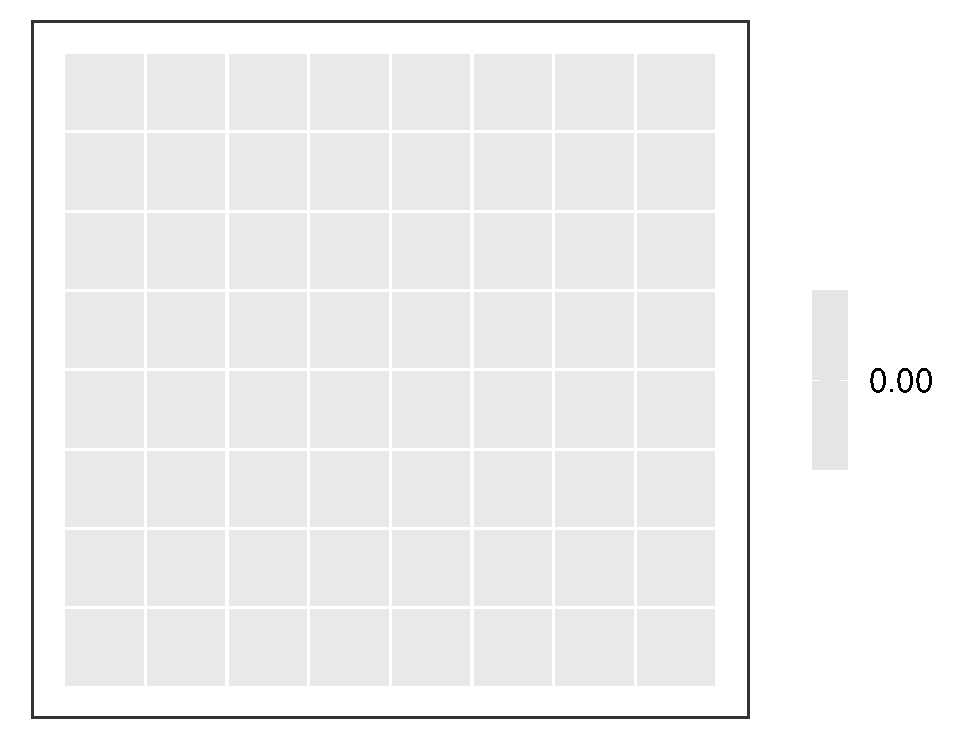
\includegraphics[height=0.8\textheight]{lecture_includes/empty_gridnoroads.pdf}
	\end{center}
\end{frame}

\begin{frame}[t]{Illustration: Market Access on a Square Island} 
\vspace{-0.3cm}
	\begin{center}
		Randomly connect adjacent regions by road \uncover<2->{and compute MA growth}

		\only<1>{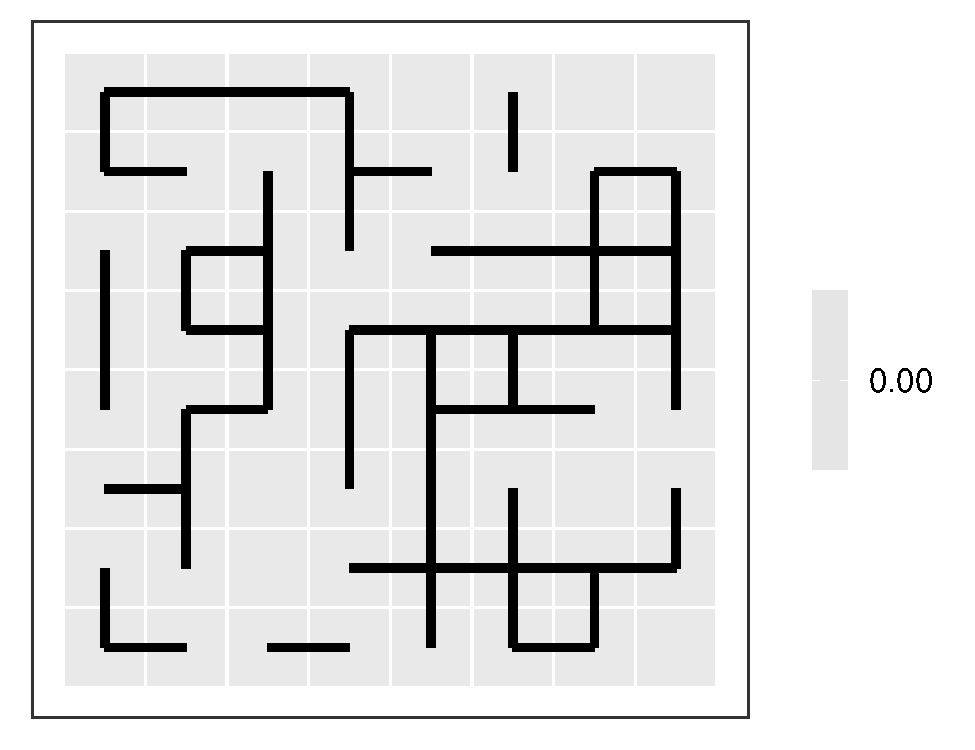
\includegraphics[height=0.8\textheight]{lecture_includes/line_only_noroads.pdf}}\only<2>{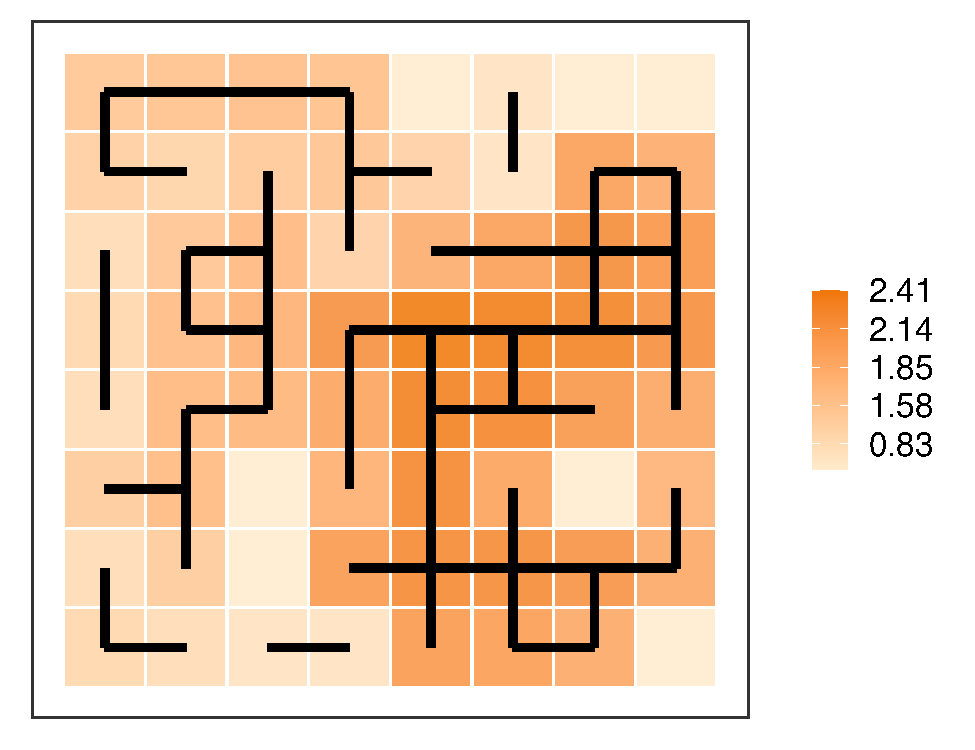
\includegraphics[height=0.8\textheight]{lecture_includes/dMA_and_line_noroads.pdf}}\only<3>{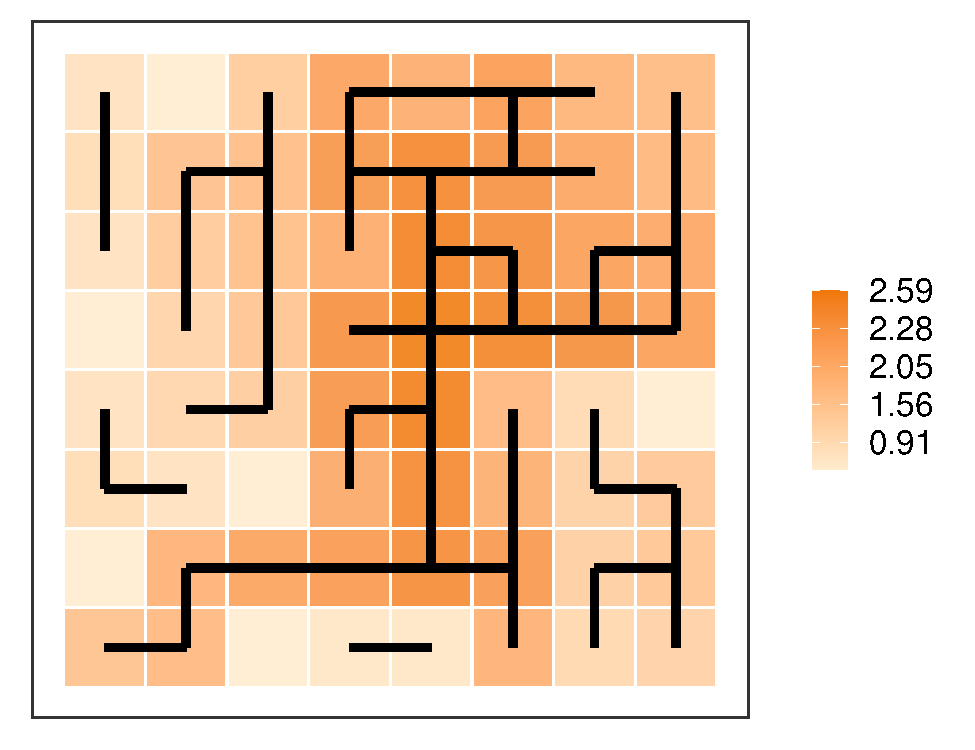
\includegraphics[height=0.8\textheight]{lecture_includes/dMA_and_line_seed2_noroads.pdf}}\only<4>{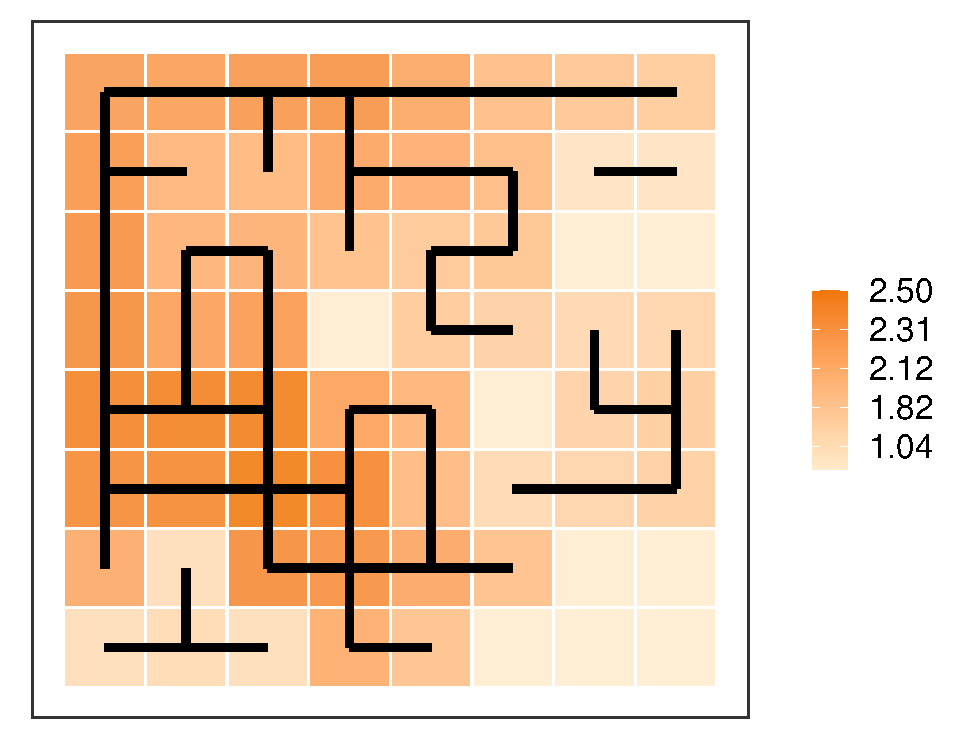
\includegraphics[height=0.8\textheight]{lecture_includes/dMA_and_line_seed3_noroads.pdf}}
	\end{center}
\end{frame}

\begin{frame}[t,label=ExpInst_noroads]{Expected Market Access Growth $\mu_i$}
\vspace{-0.3cm}
	\begin{center}
		Some regions get systematically more MA 

		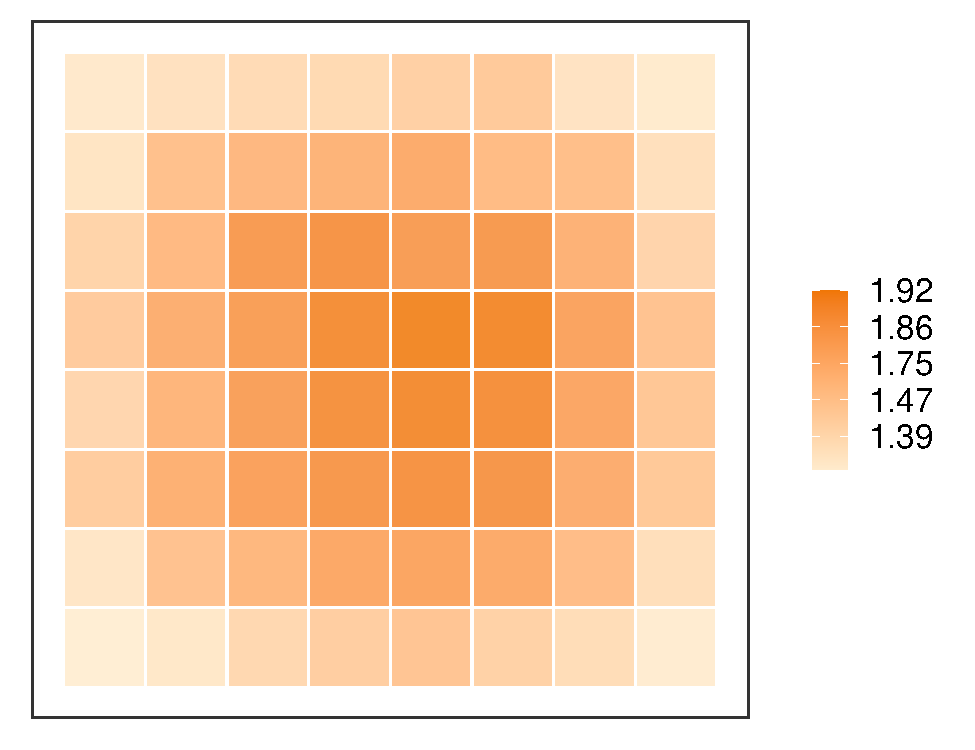
\includegraphics[height=0.8\textheight]{lecture_includes/Exp_dMA_noroads.pdf}
	\end{center}
\end{frame}

\begin{frame}[t]{Illustration: High-Speed Rail in China} 
\vspace{-0.3cm}
	\begin{center}
		149 lines were built or planned (as of April 2019)

		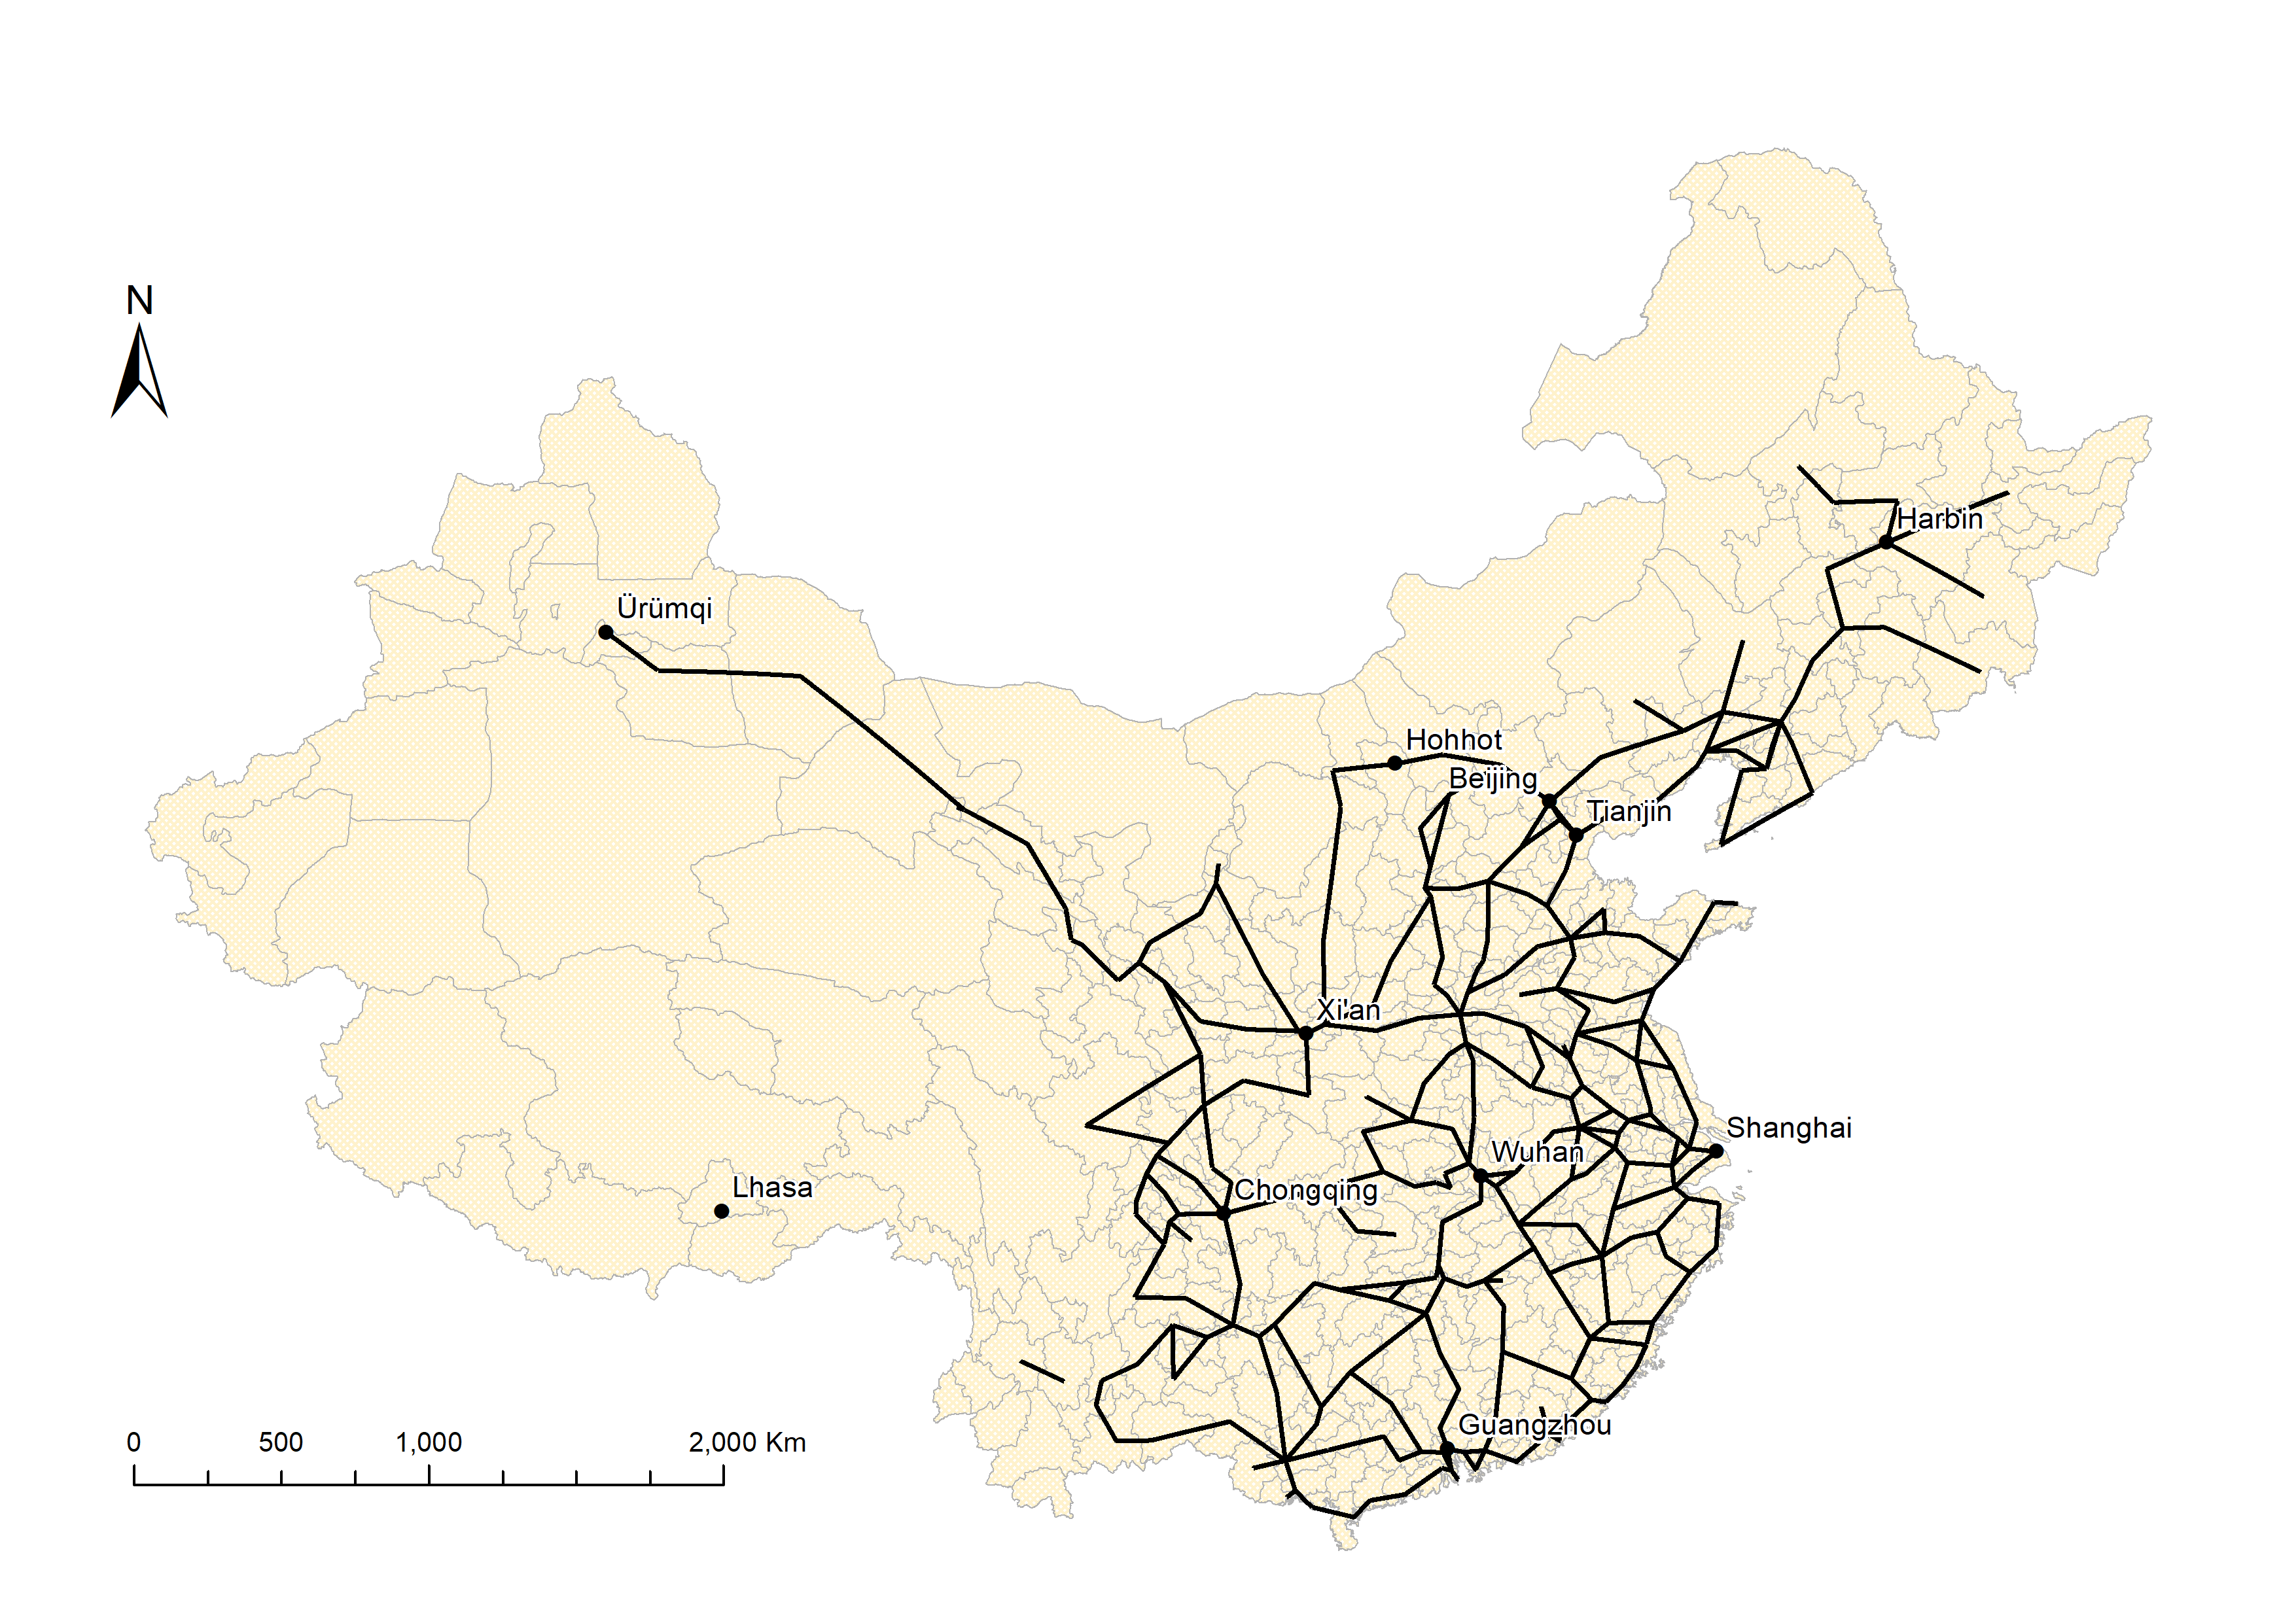
\includegraphics[trim={1cm 0.5cm 0.5cm 1cm},clip,width=11cm]{lecture_includes/Lines_actual_planned_nocolor.png}
	\end{center}
\end{frame}

\begin{frame}[t]{Illustration: High-Speed Rail in China} 
\vspace{-0.3cm}
	\begin{center}
		The 83 lines actually built by 2016. Suppose timing is random

		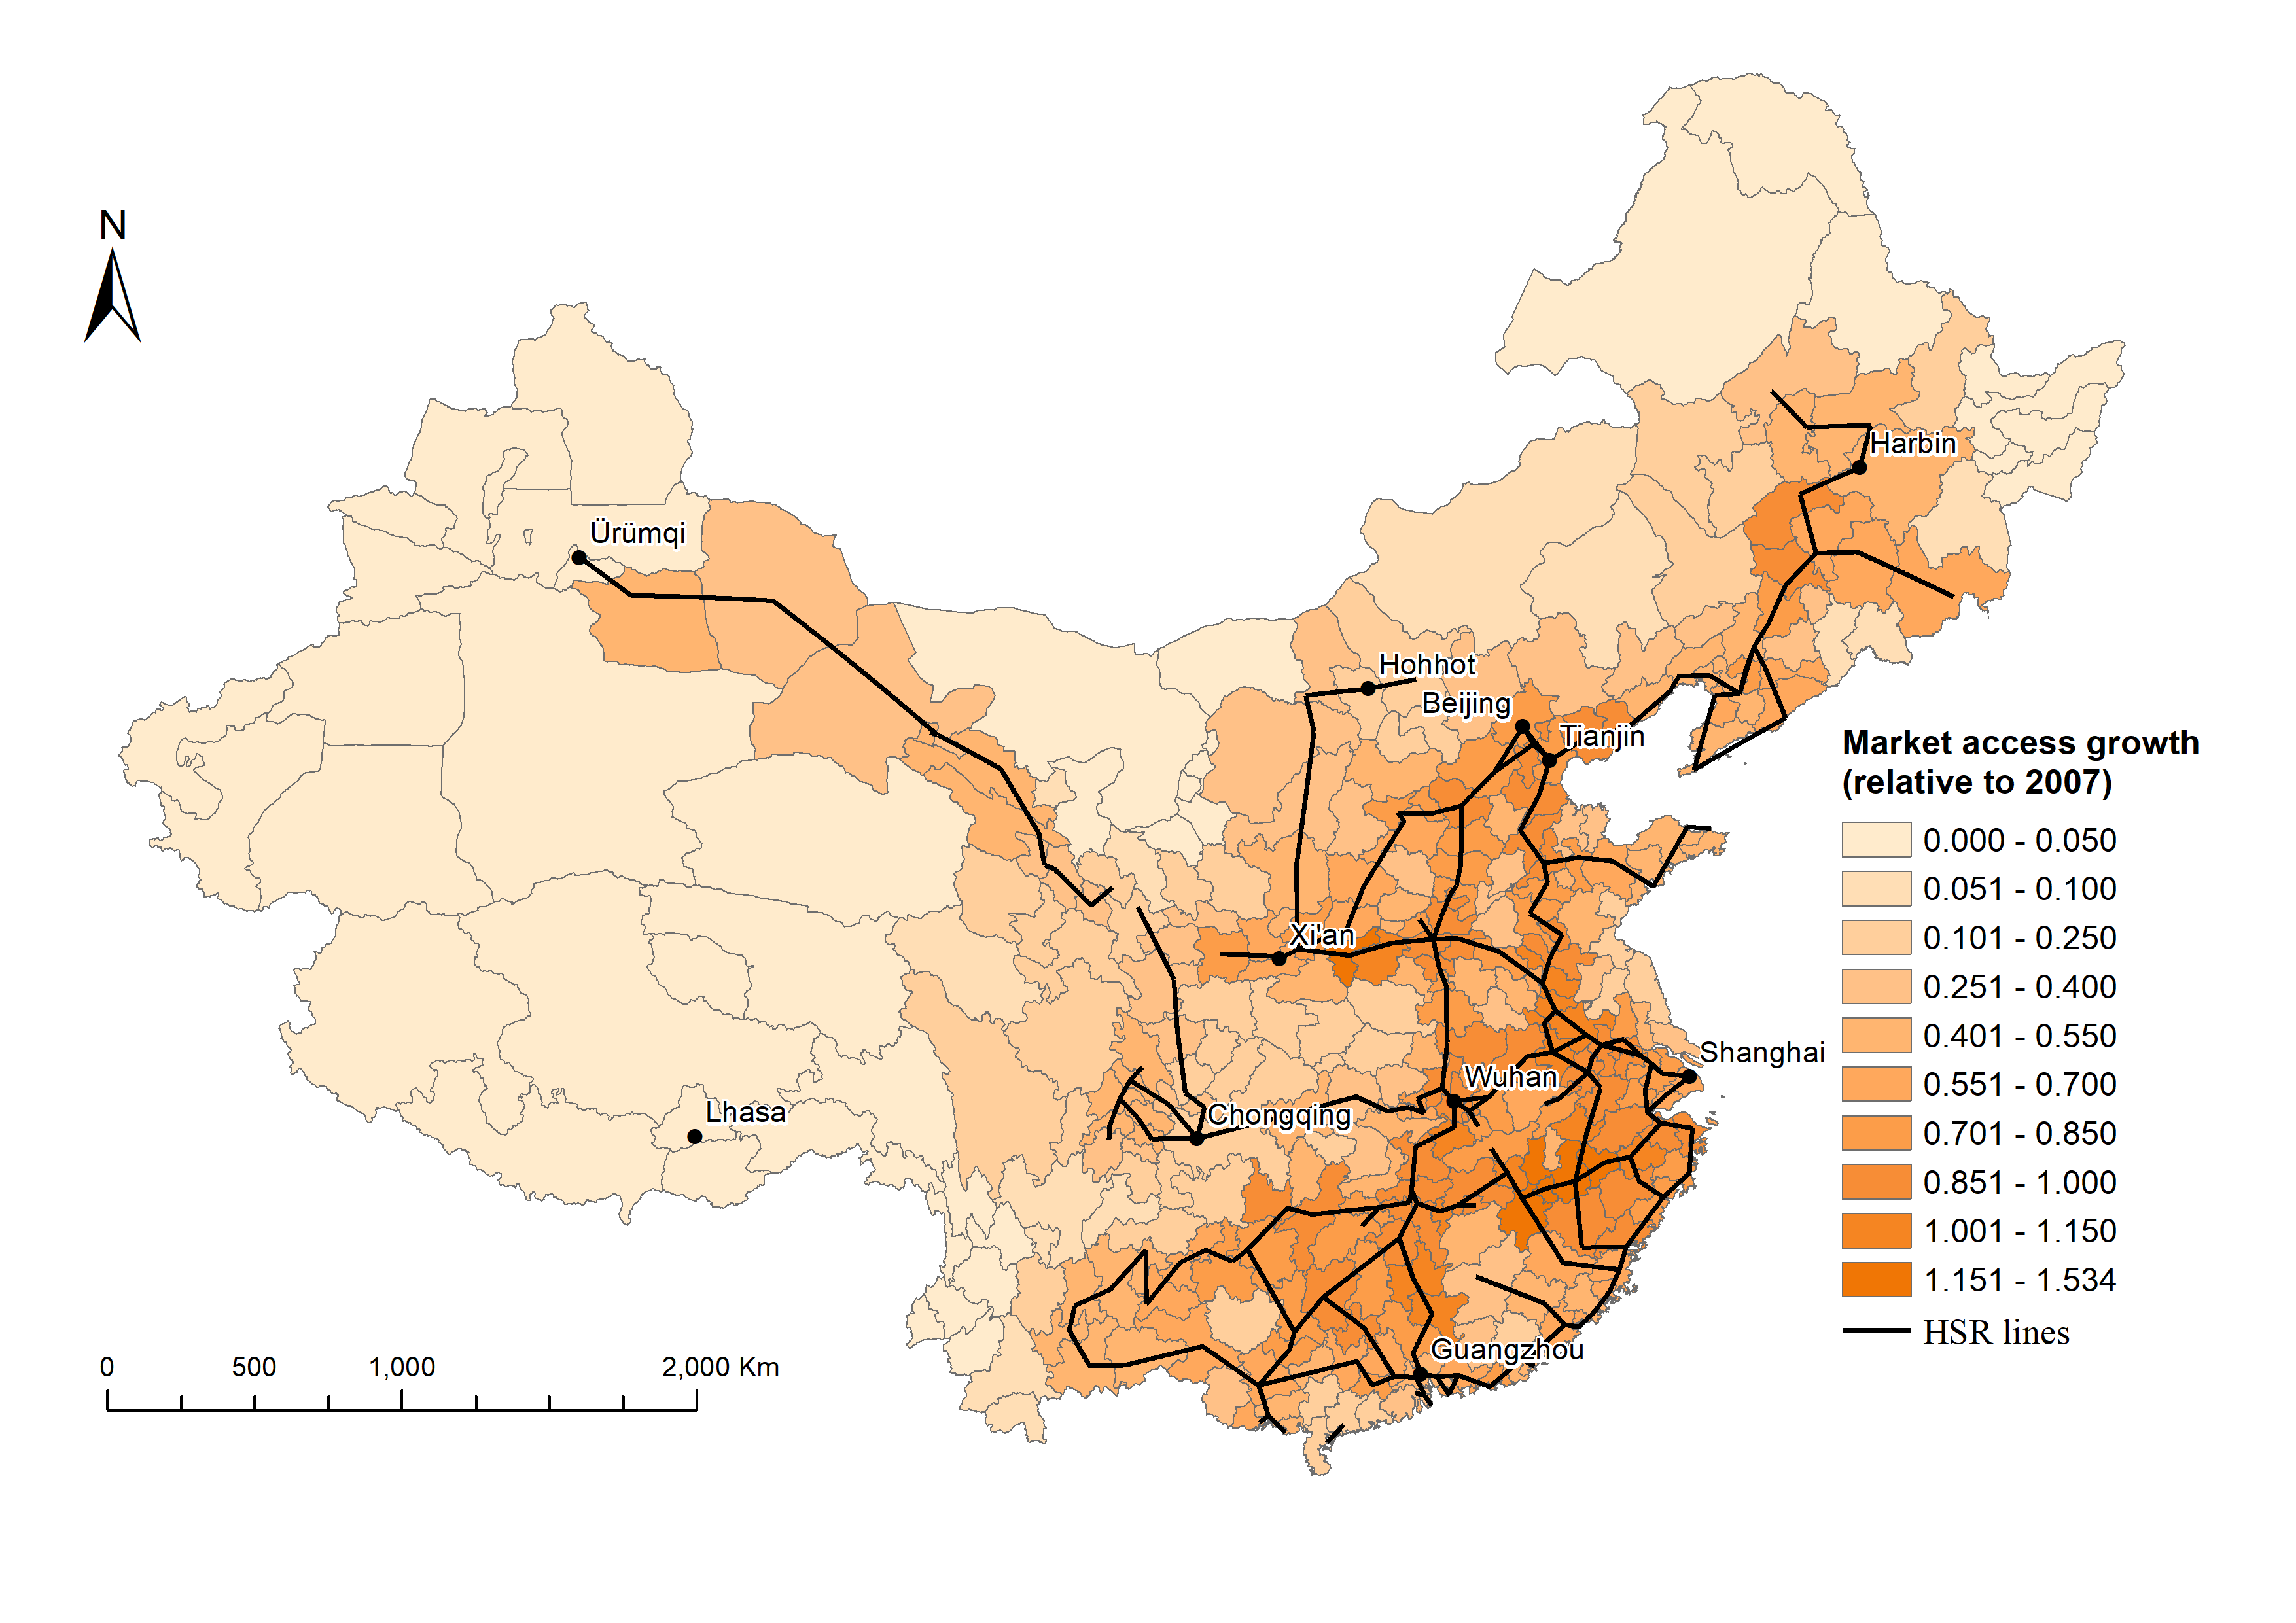
\includegraphics[trim={1cm 0.5cm 0.5cm 1cm},clip,width=11cm]{lecture_includes/Line_panel2016.png}
	\end{center}
\end{frame}

\begin{frame}[t]{Illustration: High-Speed Rail in China} 
\vspace{-0.3cm}
	\begin{center}
		A counterfactual draw of 83 lines by 2016

		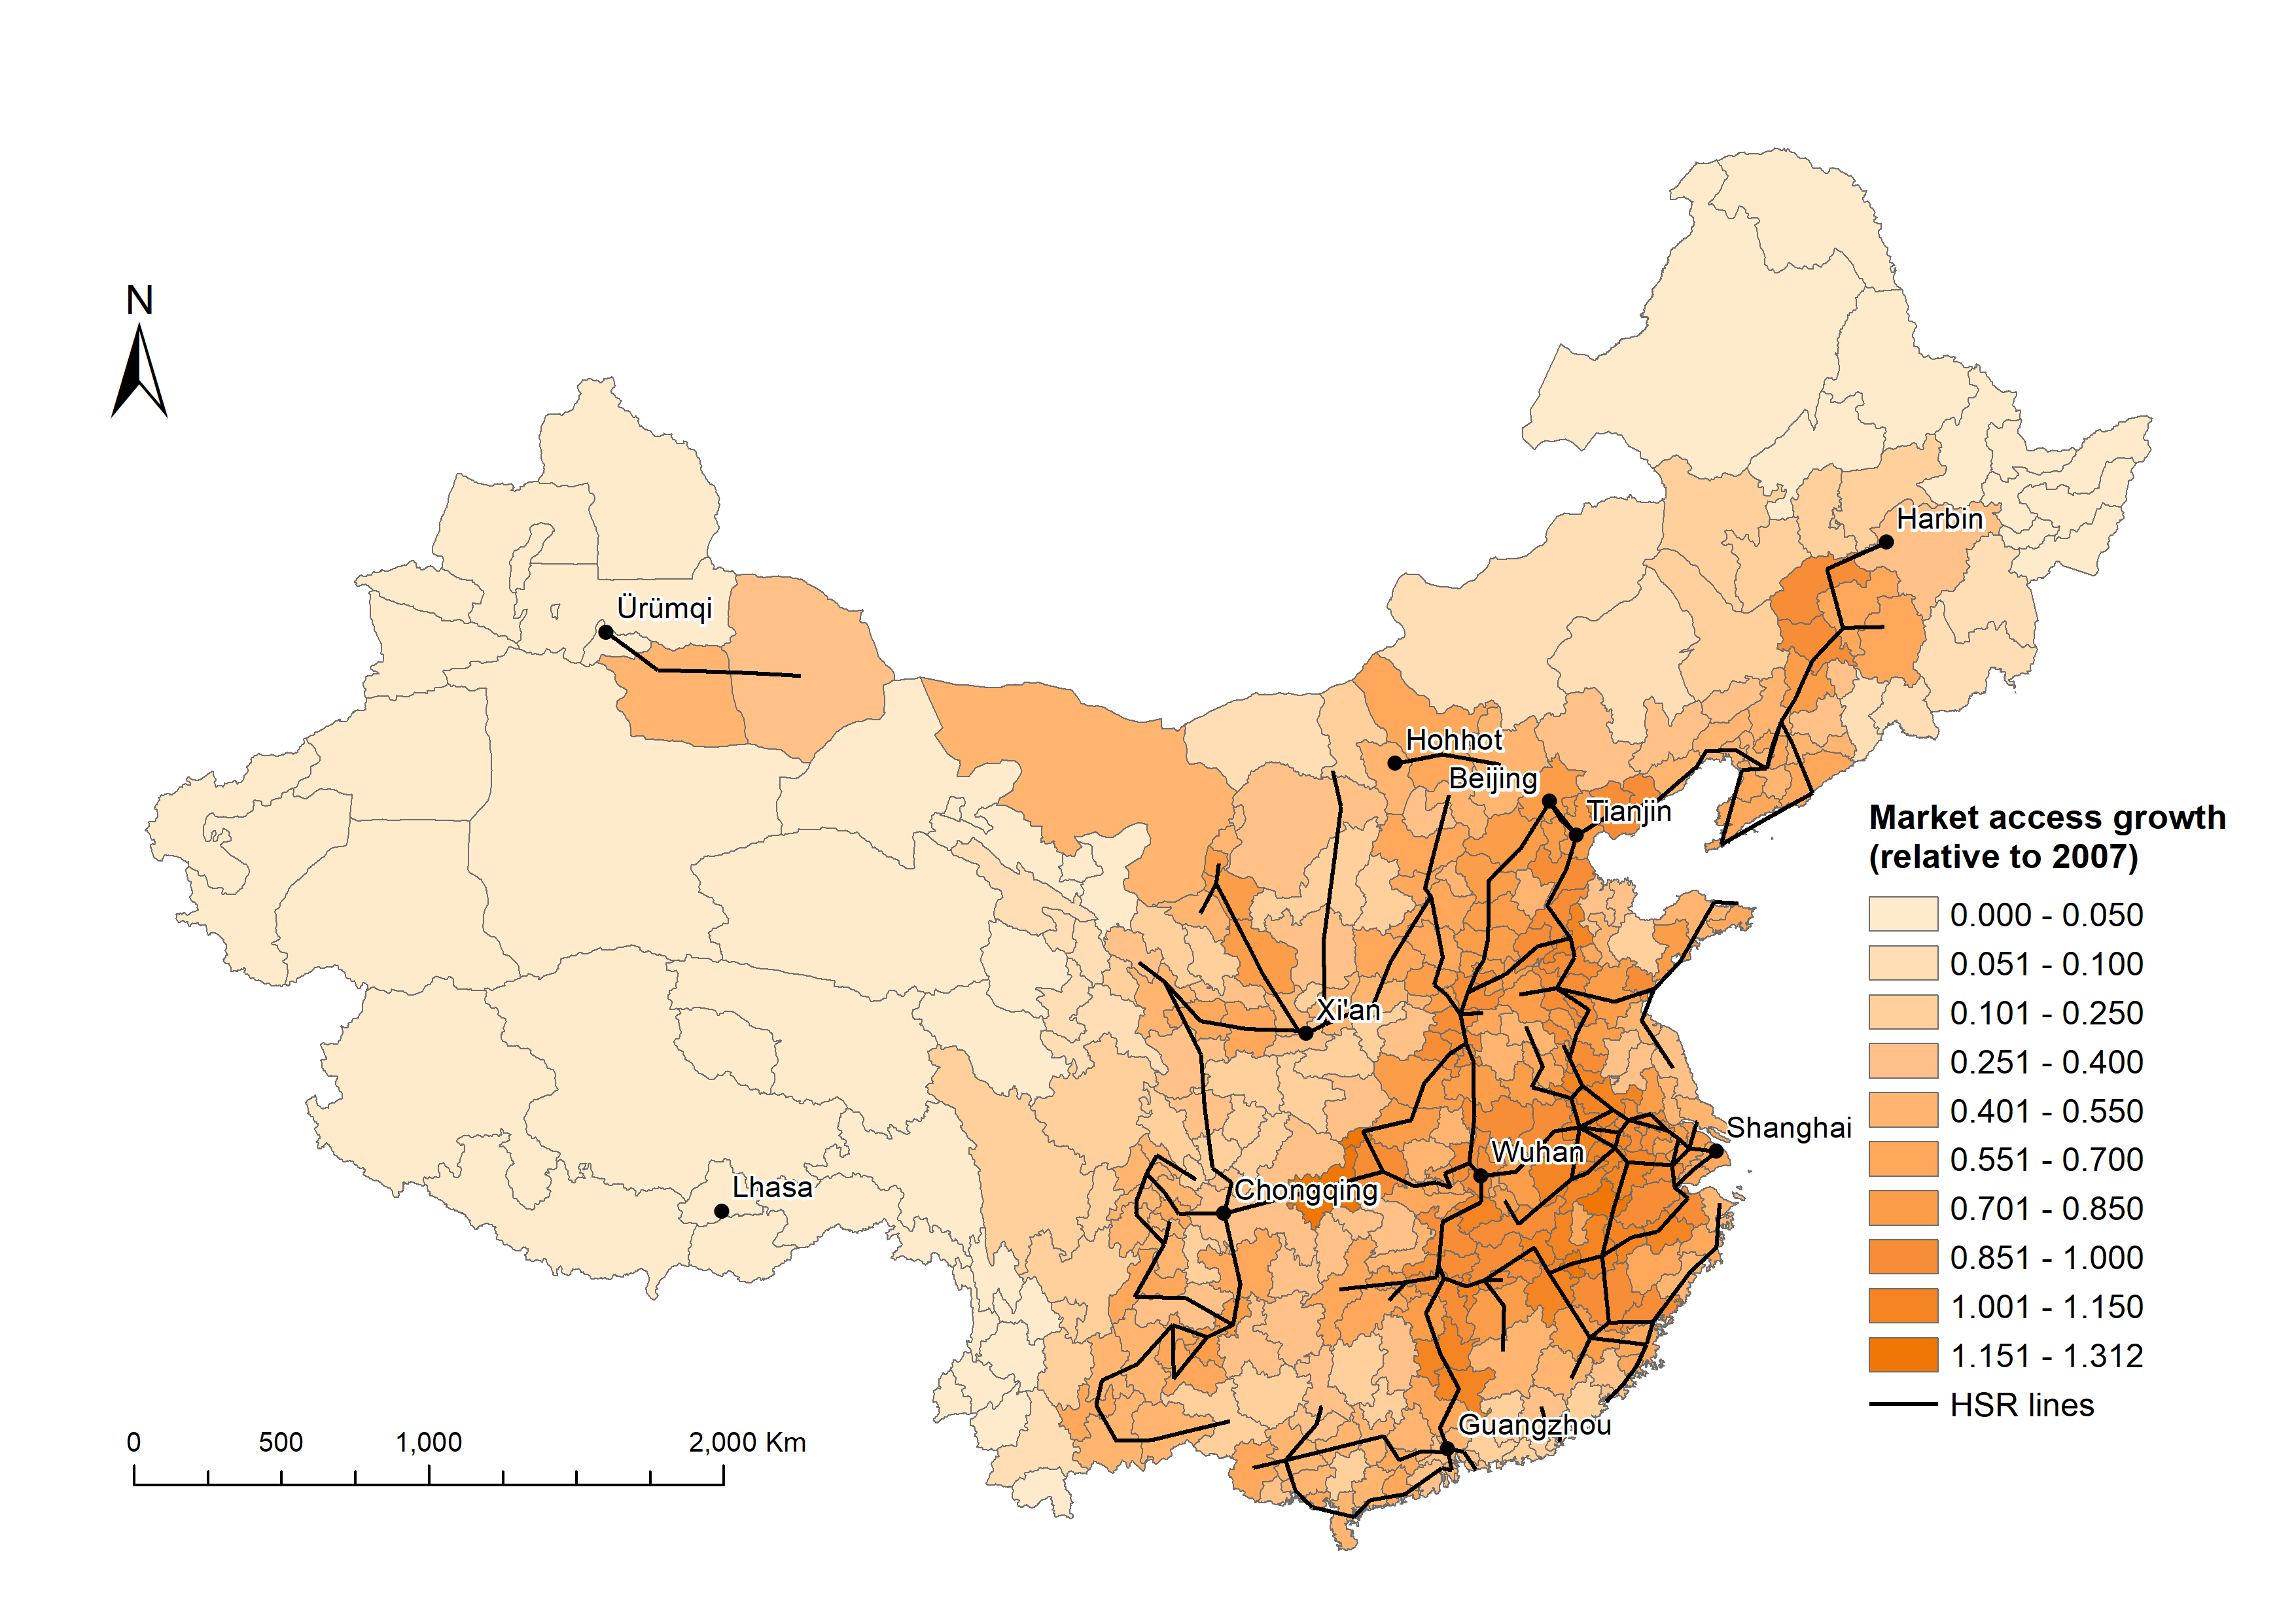
\includegraphics[trim={1cm 0.5cm 0.5cm 1cm},clip,width=11cm]{lecture_includes/Sim_Line_nlink2016.png}
	\end{center}
\end{frame}

\begin{frame}[t]{Illustration: High-Speed Rail in China} 
\vspace{-0.3cm}
	\begin{center}
		Expected MA growth, $\mu_i$

		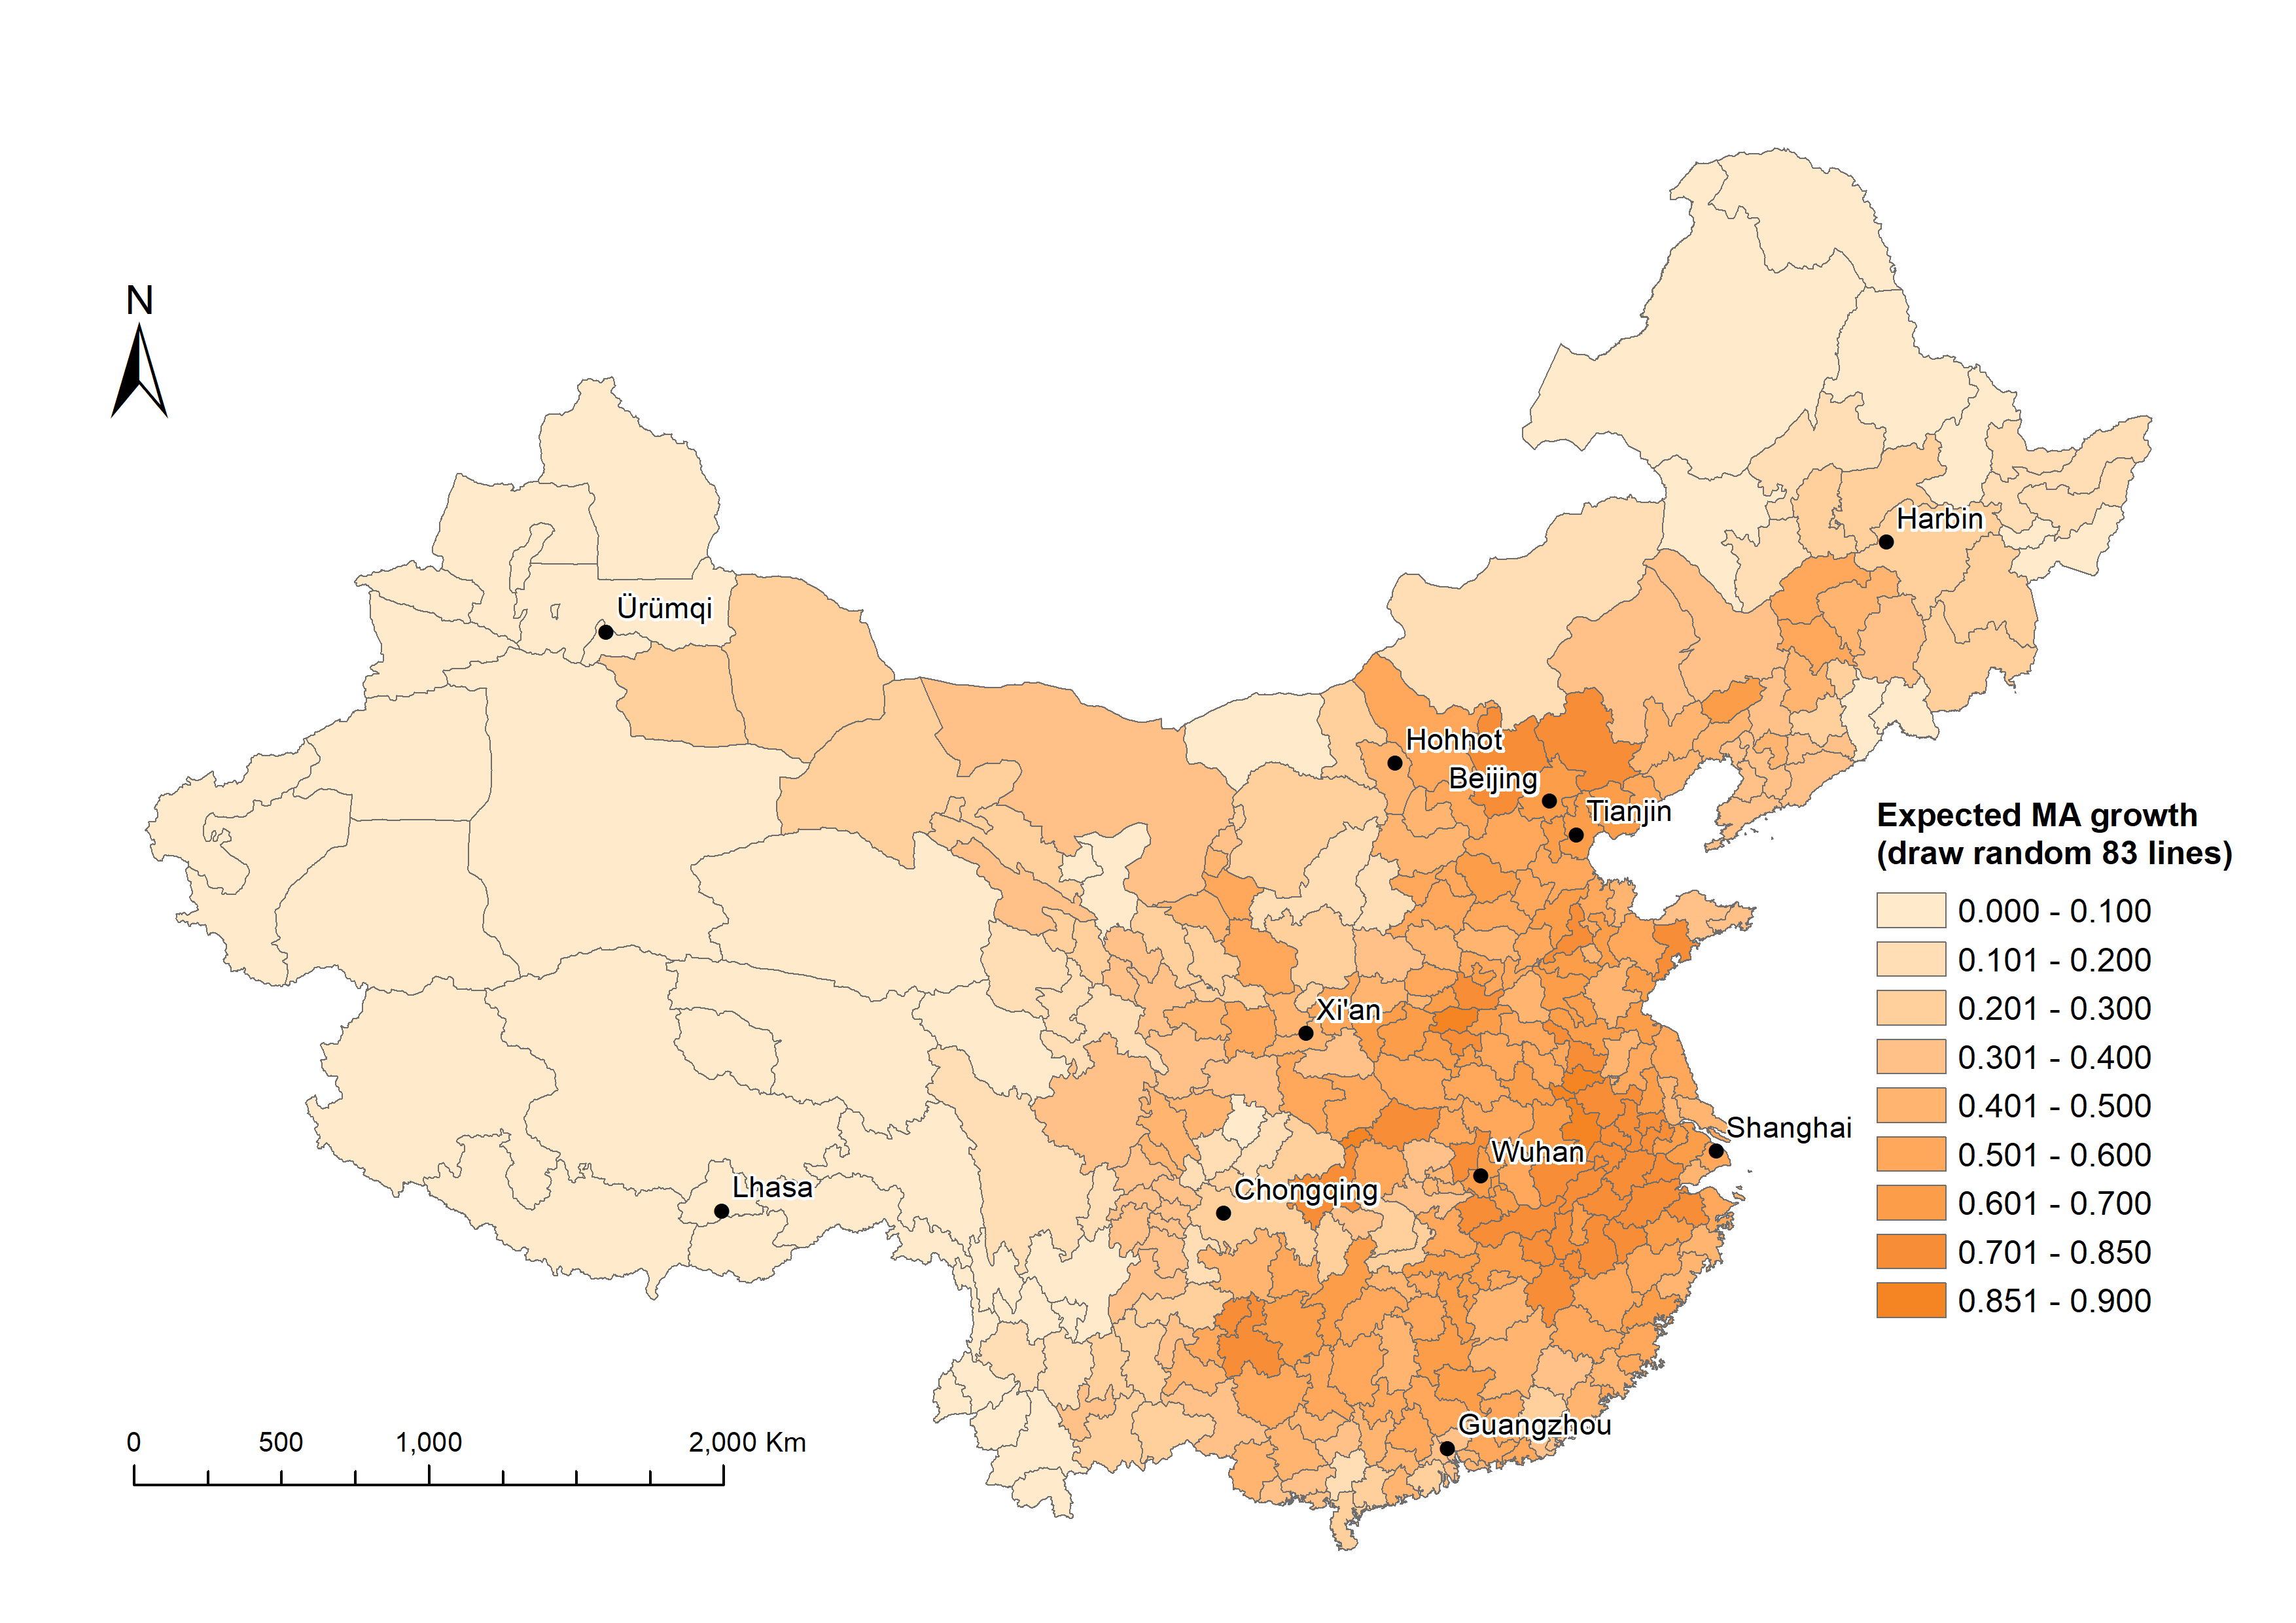
\includegraphics[trim={1cm 0.5cm 0.5cm 1cm},clip,width=11cm]{lecture_includes/DateExpected2016.png}
	\end{center}
\end{frame}

\begin{frame}[label=RCSolution]{OVB and Recentering Solution}
\vspace{0.2cm}
	Systematic variation in MA growth can generate OVB 
		\vspace{0.1cm}
		\begin{itemize}  
		\item E.g. land values fall in the periphery because of rising sea levels
		\vspace{0.1cm}
		\item More vs less developed Chinese regions may be on different trends \pause 
		\end{itemize}
	\vspace{0.5cm}
	Systematic variation can be removed via ``recentering'':\vspace{-0.25cm}
	$$\hspace{-2.85cm}\begin{matrix}\text{Recentered}\\\text{MA growth}\end{matrix}\ =\ \begin{matrix}\text{Realized}\\\text{MA growth}\end{matrix}\ -\ \begin{matrix}\text{Expected}\\\text{MA growth}\end{matrix}$$\pause
\vspace{-0.2cm}

Recentered MA is a valid instrument for realized MA growth 
		\vspace{0.1cm}
		\begin{itemize}  
		\item Compares MA from actual and counterfactual shocks 
		\end{itemize}
\end{frame}

\subsection{Medicaid Eligibility Effects}
\begin{frame}{Example 2: Effects of Program Eligibility}
Consider the effects of individual eligilibity $x_i$ for Medicaid:
$$y_i=\beta x_i+\varepsilon_i$$ 
where $x_i$ is determined by $i$'s state policy ${\color<2->{sun}g}{}_{\color<3->{electric-violet}\text{state}_i}$ and {\color<3->{electric-violet}demographics}\pause
\vspace{0.05cm}
	\begin{itemize}
	\item Suppose \bgSun{state policies} are as-good-as-random 
	\vspace{0.1cm}\pause
	\item But \bgElectricViolet{pre-determined demographics} are endogeous $\Rightarrow$ OLS biased
	\end{itemize}
\vspace{0.3cm}\pause
Standard ``simulated instruments'' solution (Currie and Gruber (1996)): \\ use state-level variation (a measure of policy generosity) as IV for $x_i$ 

\begin{itemize}
\item This works, but is likely inefficient: policy shocks have heterogeneous effects across individuals
\end{itemize}
\end{frame}

\begin{frame}{Gaining Power from Recentering}
Consider the effects of individual eligilibity $x_i$ for Medicaid:
$$y_i=\beta x_i+\varepsilon_i$$ 
where $x_i$ is determined by $i$'s state policy ${\color{sun}g}{}_{\color{electric-violet}\text{state}_i}$ and {\color{electric-violet}demographics}\pause
\vspace{0.3cm}\pause
The BH approach:
\vspace{0.05cm}
	\begin{itemize}
	\item Formalize the policy experiment as ``all permutations of $\color{sun}g$ across states are equally likely''
	\vspace{0.1cm}\pause
	\item Compute $\mu_i$ = the share of states in which $i$ would be eligible
	\vspace{0.1cm}\pause
	\item Leverage all variation in $x_i$ but recenter by $\mu_i$ (or control for $\mu_i$)
	\vspace{0.1cm}\pause
	\item Yields efficiency gain by better first-stage prediction, e.g. by removing $i$ who are always or never eligible 
	\end{itemize}
\end{frame}

\section{Formal Framework}

\begin{frame}{General Setup}

\vspace{-0.2cm}
We have a model of $y_i=\beta x_i+\varepsilon_i $ for a fixed population $i=1\dots N$
\begin{itemize}
\item In BH: extensions to heterogeneous effects, other controls, multiple treatments, nonlinear outcome models, panel data...
\end{itemize}

\pause\vspace{0.2cm}
We have a candidate instrument $z_i = f_i ({\color{sun}g},{\color{electric-violet}w})$, where {\color{sun} $g$} is a vector of shocks; {\color{electric-violet} $w$} collects predetermined variables; $f_i(\cdot)$ are known mappings 
	\begin{itemize}
	\item Applies to any $z_i$ which can be constructed from observed data
	\item Nests reduced-form regressions: $x_i=z_i$
	\item Allows ${\color{sun} g}=({\color{sun} g_1},\dots,{\color{sun} g_K})$ to vary at a different level than $i$
	\end{itemize}

\pause\vspace{0.2cm}
\textbf{Assumptions}:
	\begin{enumerate}
	\item Shocks are exogenous: ${\color{sun}g} \perp \varepsilon \mid {\color{electric-violet} w}$
	\item Conditional distribution $G({\color{sun}g}\mid{\color{electric-violet} w})$ is known (e.g. via randomization protocol or uniform across permutations of $\color{sun}g$)
	\end{enumerate}

\end{frame}

\begin{frame}{Main Results}
	The expected instrument, $\mu_i=E[f_i({\color{sun}g},{\color{electric-violet}w})\mid {\color{electric-violet}w}]\equiv\int f_i({\color{sun}g},{\color{electric-violet}w})dG({\color{sun}g}\mid {\color{electric-violet}w})$, is the sole confounder generating OVB:
%	\vspace{-0.1cm}
	$$E\left[\frac{1}{N}\sum_i z_i \varepsilon_i\right]=E\left[\frac{1}{N}\sum_i\mu_i \varepsilon_i\right]\ne 0\text{, in general}$$
	\pause\vspace{-0.2cm}
	The \emph{recentered instrument} $\tilde{z}_i=z_i-\mu_i$ is a valid instrument for $x_i$:
%	\vspace{-0.1cm}
	$$E\left[\frac{1}{N}\sum_i \tilde z_i \varepsilon_i\right]=0$$ % provided it has a first stage
%	It thus identifies $\beta$, given a first stage ($\expec{\frac{1}{L}\sum_i \tilde z_i x_i}\neq 0$)
	\pause
	Regressions which control for $\mu_i$ also identify $\beta$ (implicitly recenter, by the FWL theorem)
\end{frame}

\begin{frame}{Extensions}
	\textbf{Consistency}: follows when $\tilde z_i$ is weakly mutually dependent across $i$
	\vspace{0.25cm}

	 \textbf{Robustness} to heterogeneous treatment effects: $\tilde{z}_i$ identifies a convex avg. of $\beta_i$ under appropriate first-stage monotonicity
	\vspace{0.25cm}

	 \textbf{Randomization inference} provides exact confidence intervals for $\beta$ (under constant effects) and falsification tests 
	\vspace{0.25cm}

	BH also characterize the \textbf{asy.~efficient} recentered IV among all $f_i(\cdot)$ 

\end{frame}

\section{Applications}

\subsection{Market Access Effects}
\begin{frame}[label=HSRApplication]{App. 1: Market Access from Chinese High-Speed Rail}
	We first show how instrument recentering can address OVB when estimating the effects of market access growth
	
	\vspace{0.4cm}
	\textbf{Setting}: Chinese HSR; 83 lines built 2008--2016, 66 yet unbuilt
	\vspace{0.1cm}
	\begin{itemize}
	\item Market access: $MA_{i t}= \sum_k \exp\left(-0.02\tau_{i k t}\right) p_{k,2000}$, where $\tau_{i k t}$ is HSR-affected travel time between prefecture capitals (Zheng and Kahn, 2013) and $p_{i,2000}$ is prefecture $i$'s population in 2000
	\vspace{0.1cm}
	\item Relate to employment growth in 274 prefectures, 2007-2016
	\end{itemize}
\end{frame}
	

\begin{frame}{Simple OLS Regressions Suggest a Large MA Effect} 
	\begin{center}
	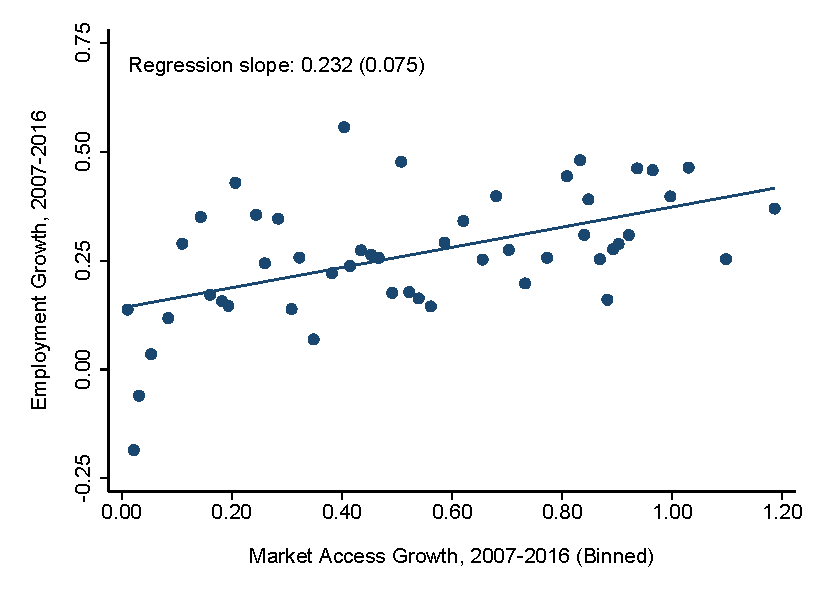
\includegraphics[width=\textwidth]{lecture_includes/emp_ols_binscatter.pdf}
	\end{center}
\end{frame}

\begin{frame}[t,label=LinePanel]{High vs. Low MA Growth is Not a Convincing Contrast!}
	\begin{center}
	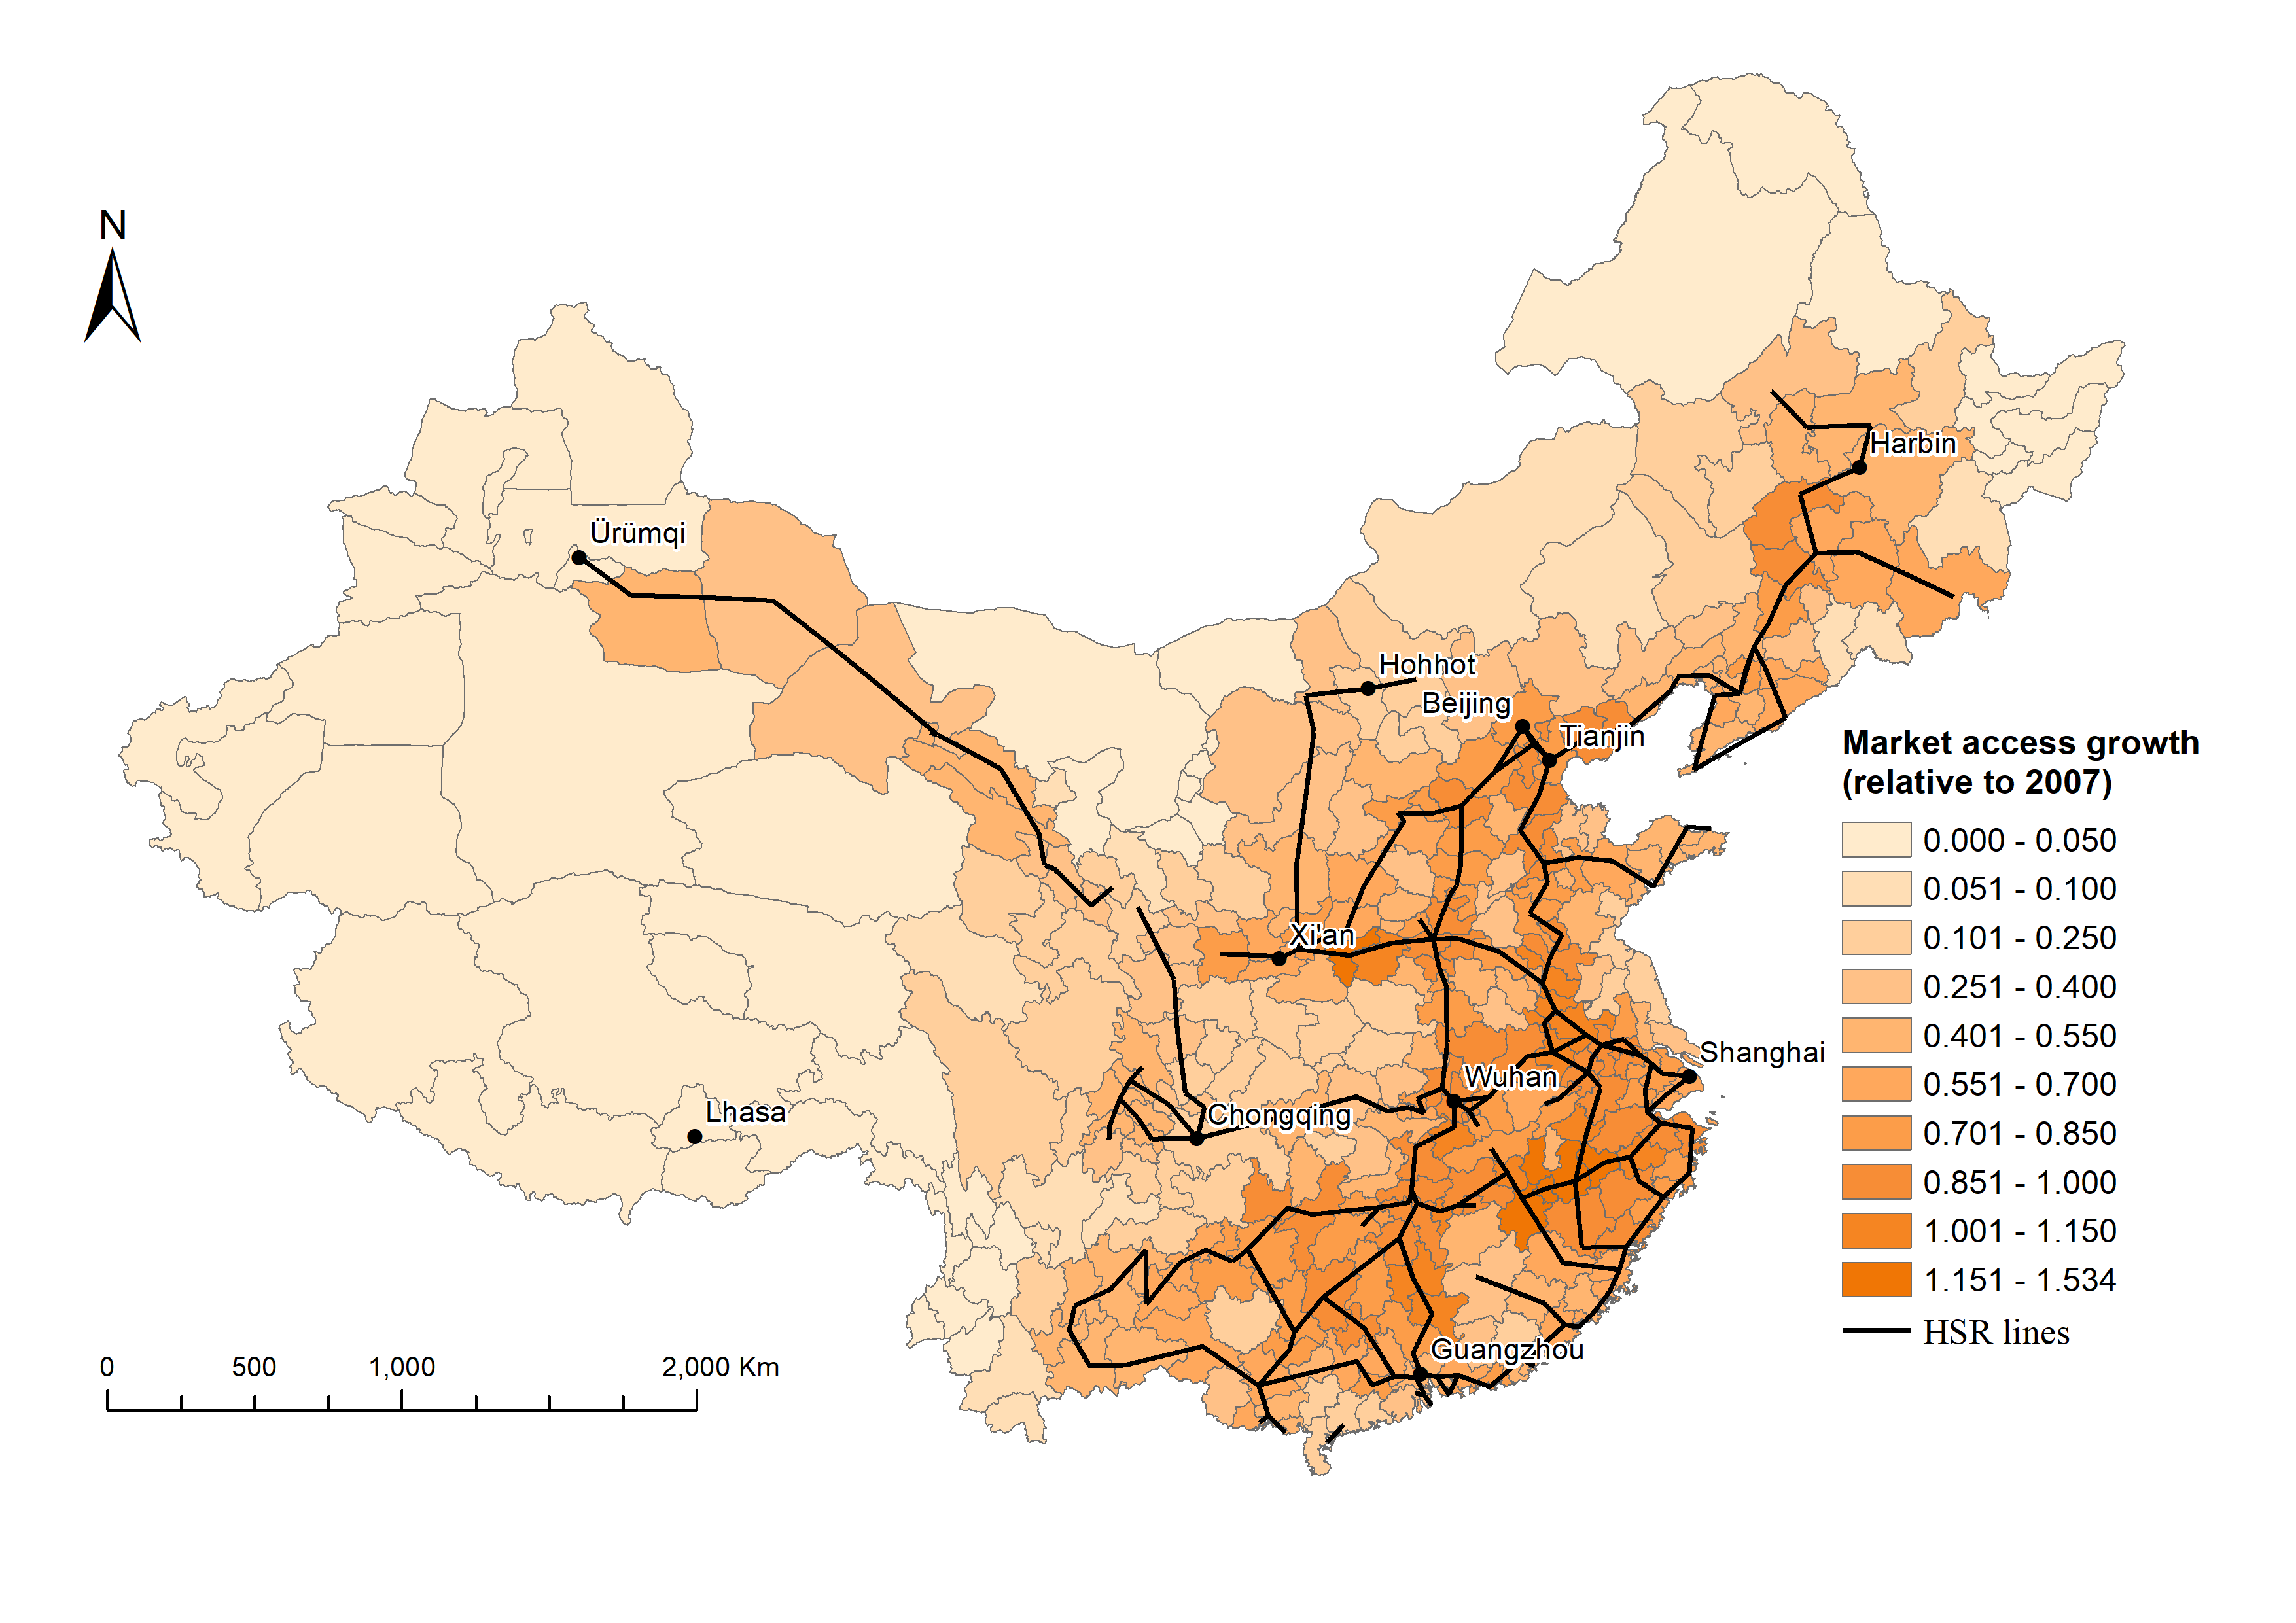
\includegraphics[trim={1cm 0.5cm 0.5cm 1cm},clip,width=11cm]{lecture_includes/Line_panel2016.png}
	\end{center}
\end{frame}

\begin{frame}[label=HSR]{How to Find Valid Treatment-Control Contrasts?}
Add controls (province FE, longitude, etc...)
\vspace{0.05cm}
	\begin{itemize}
	\item Hard to justify \emph{ex ante} since MA is a constructed variable 
	\vspace{0.1cm}
	\item No experimental analog
	\end{itemize}
\vspace{0.4cm}\pause
Find valid contrasts for \emph{one} source of variation---a natural experiment
\vspace{0.05cm}
	\begin{itemize}
	\item Bartelme (2018): shocks affecting market size
	\vspace{0.1cm}
	\item Donaldson (2018): built vs unbuilt lines
	\vspace{0.1cm}
	\item BH application: assume random timing of observably similar lines 
	\end{itemize}
\end{frame}

\begin{frame}[t,label=BuiltPlanned]{Built and Planned HSR Lines}
\vspace{-0.5cm}
	\begin{center}
	BH reshuffle built \& planned lines connecting the same \# of regions 
	
	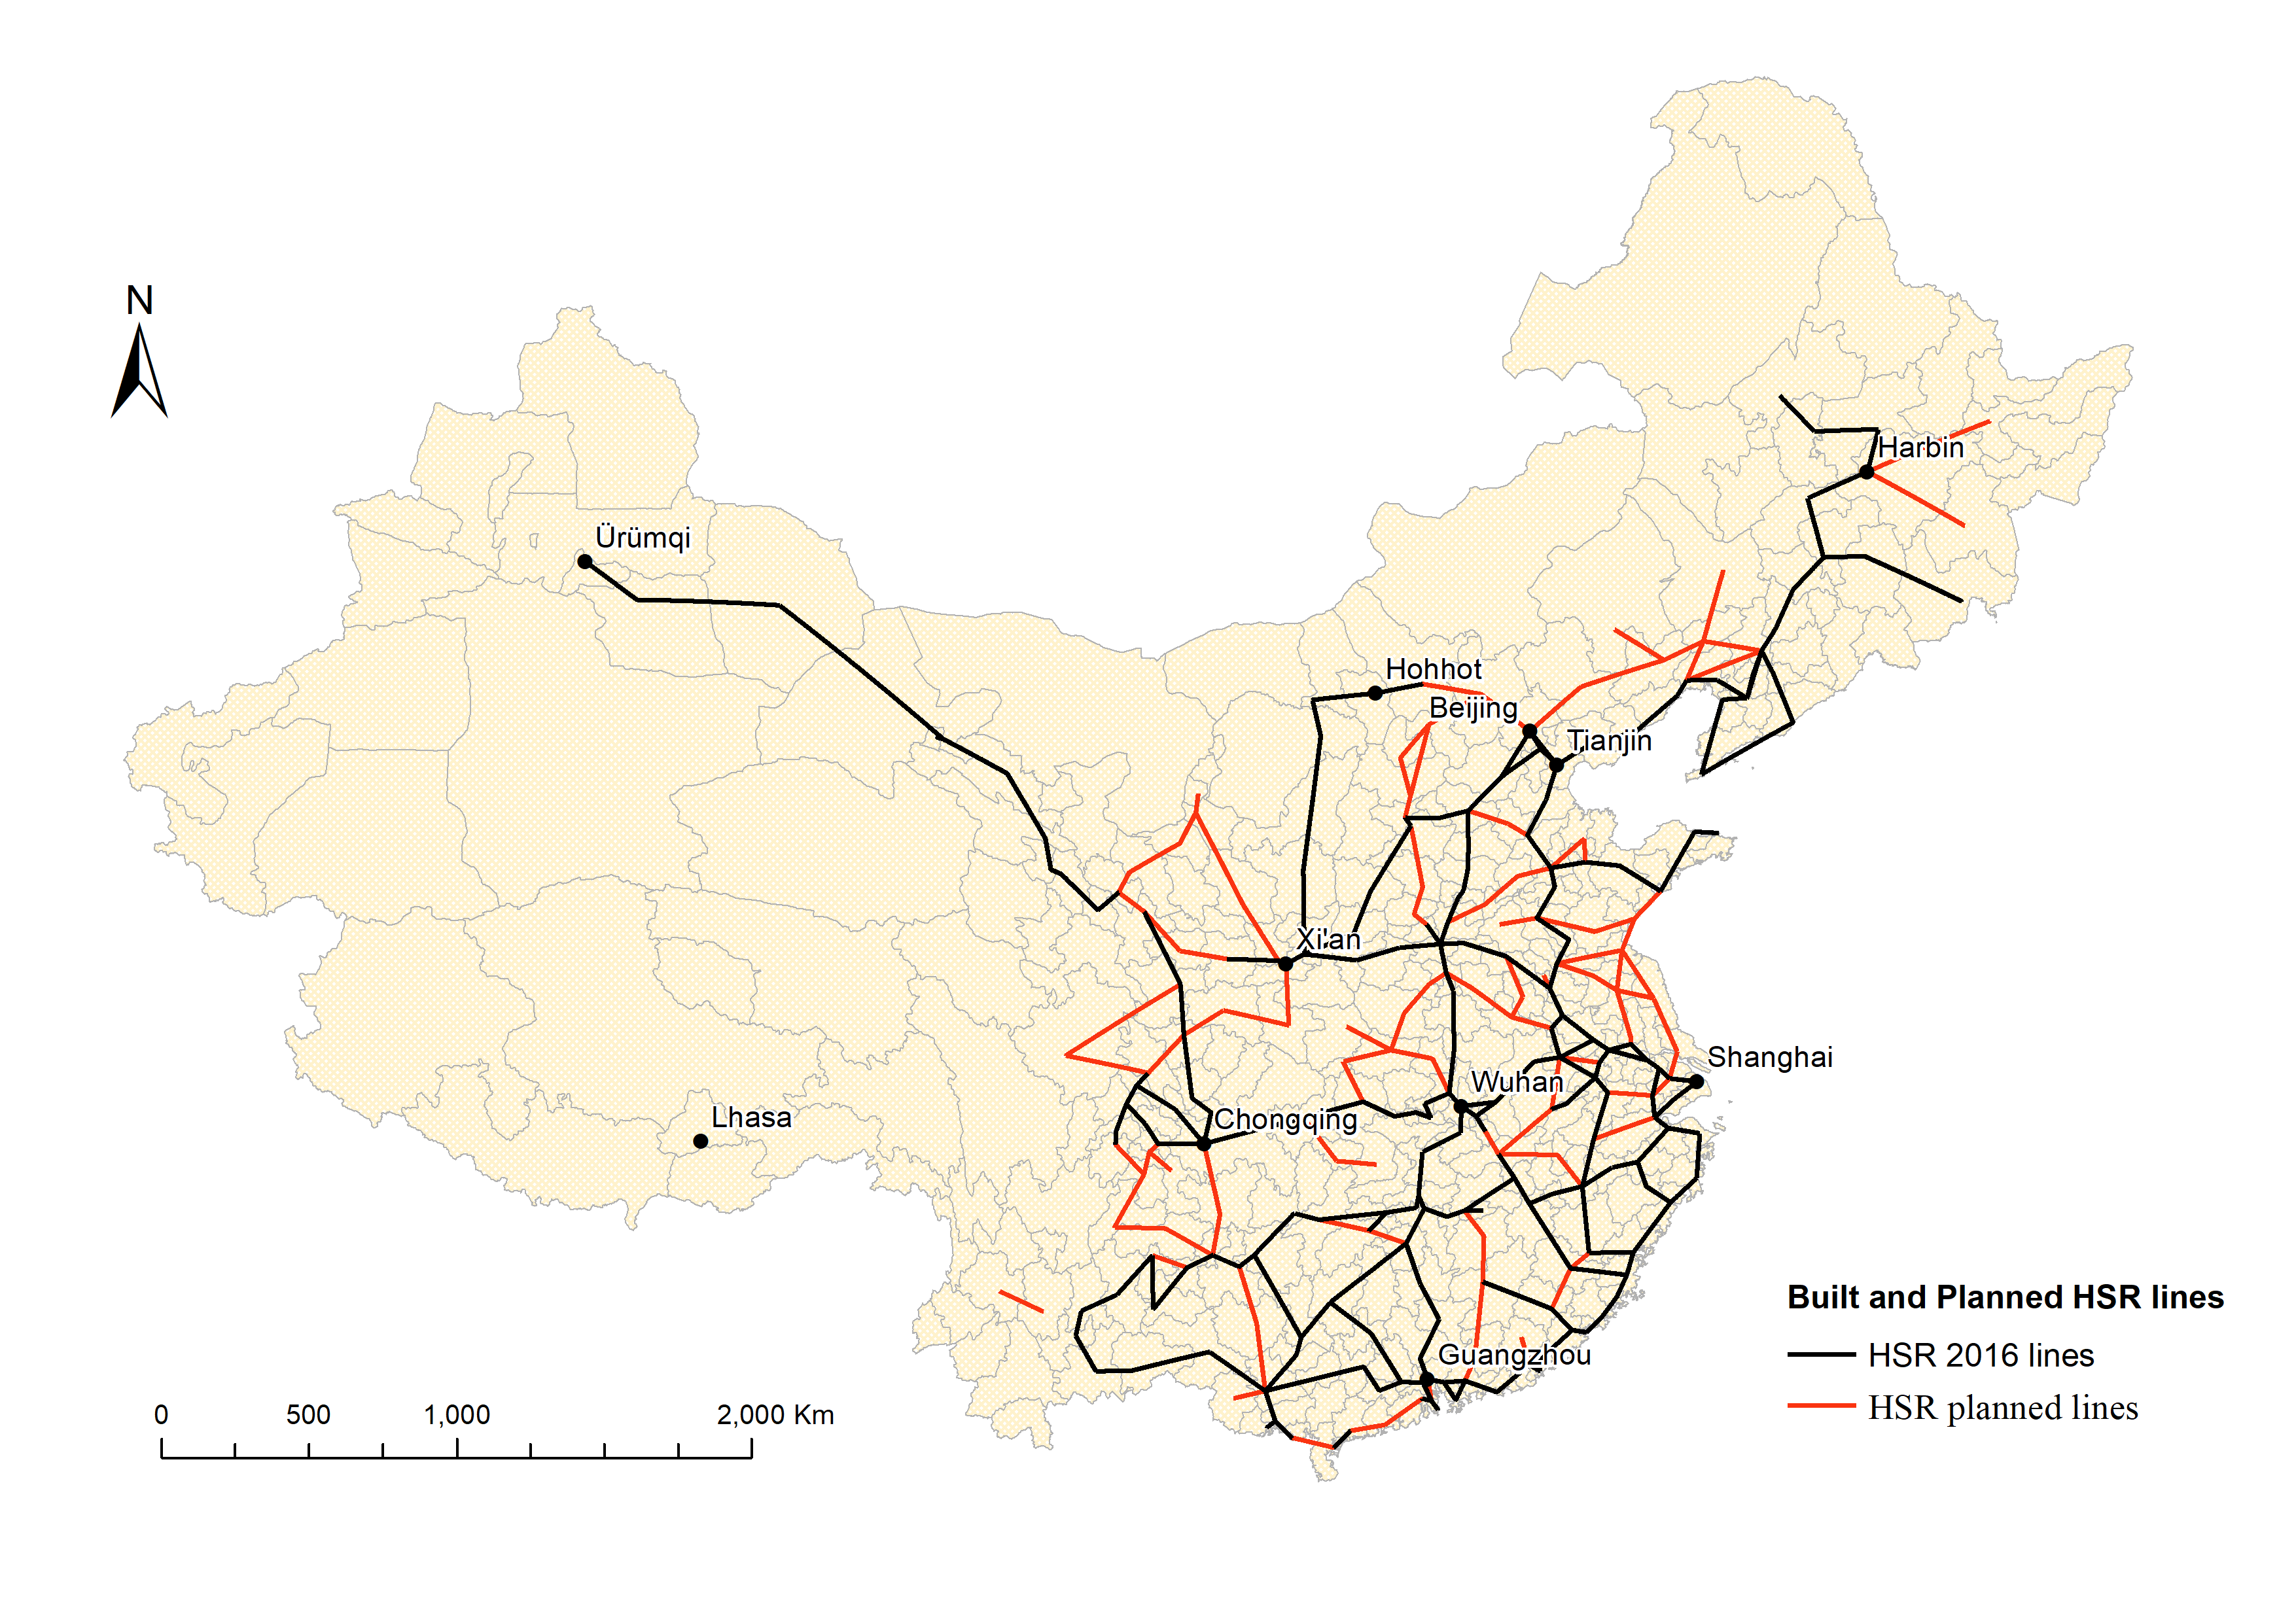
\includegraphics[trim={1cm 0.5cm 0.5cm 1cm},clip,width=11cm]{lecture_includes/Lines_actual_planned.png}
	\end{center}
\end{frame}

\begin{frame}[t,label=HSRExpected]{Expected Market Access Growth (2007--2016), $\mu_i$}
	\begin{center}
	
	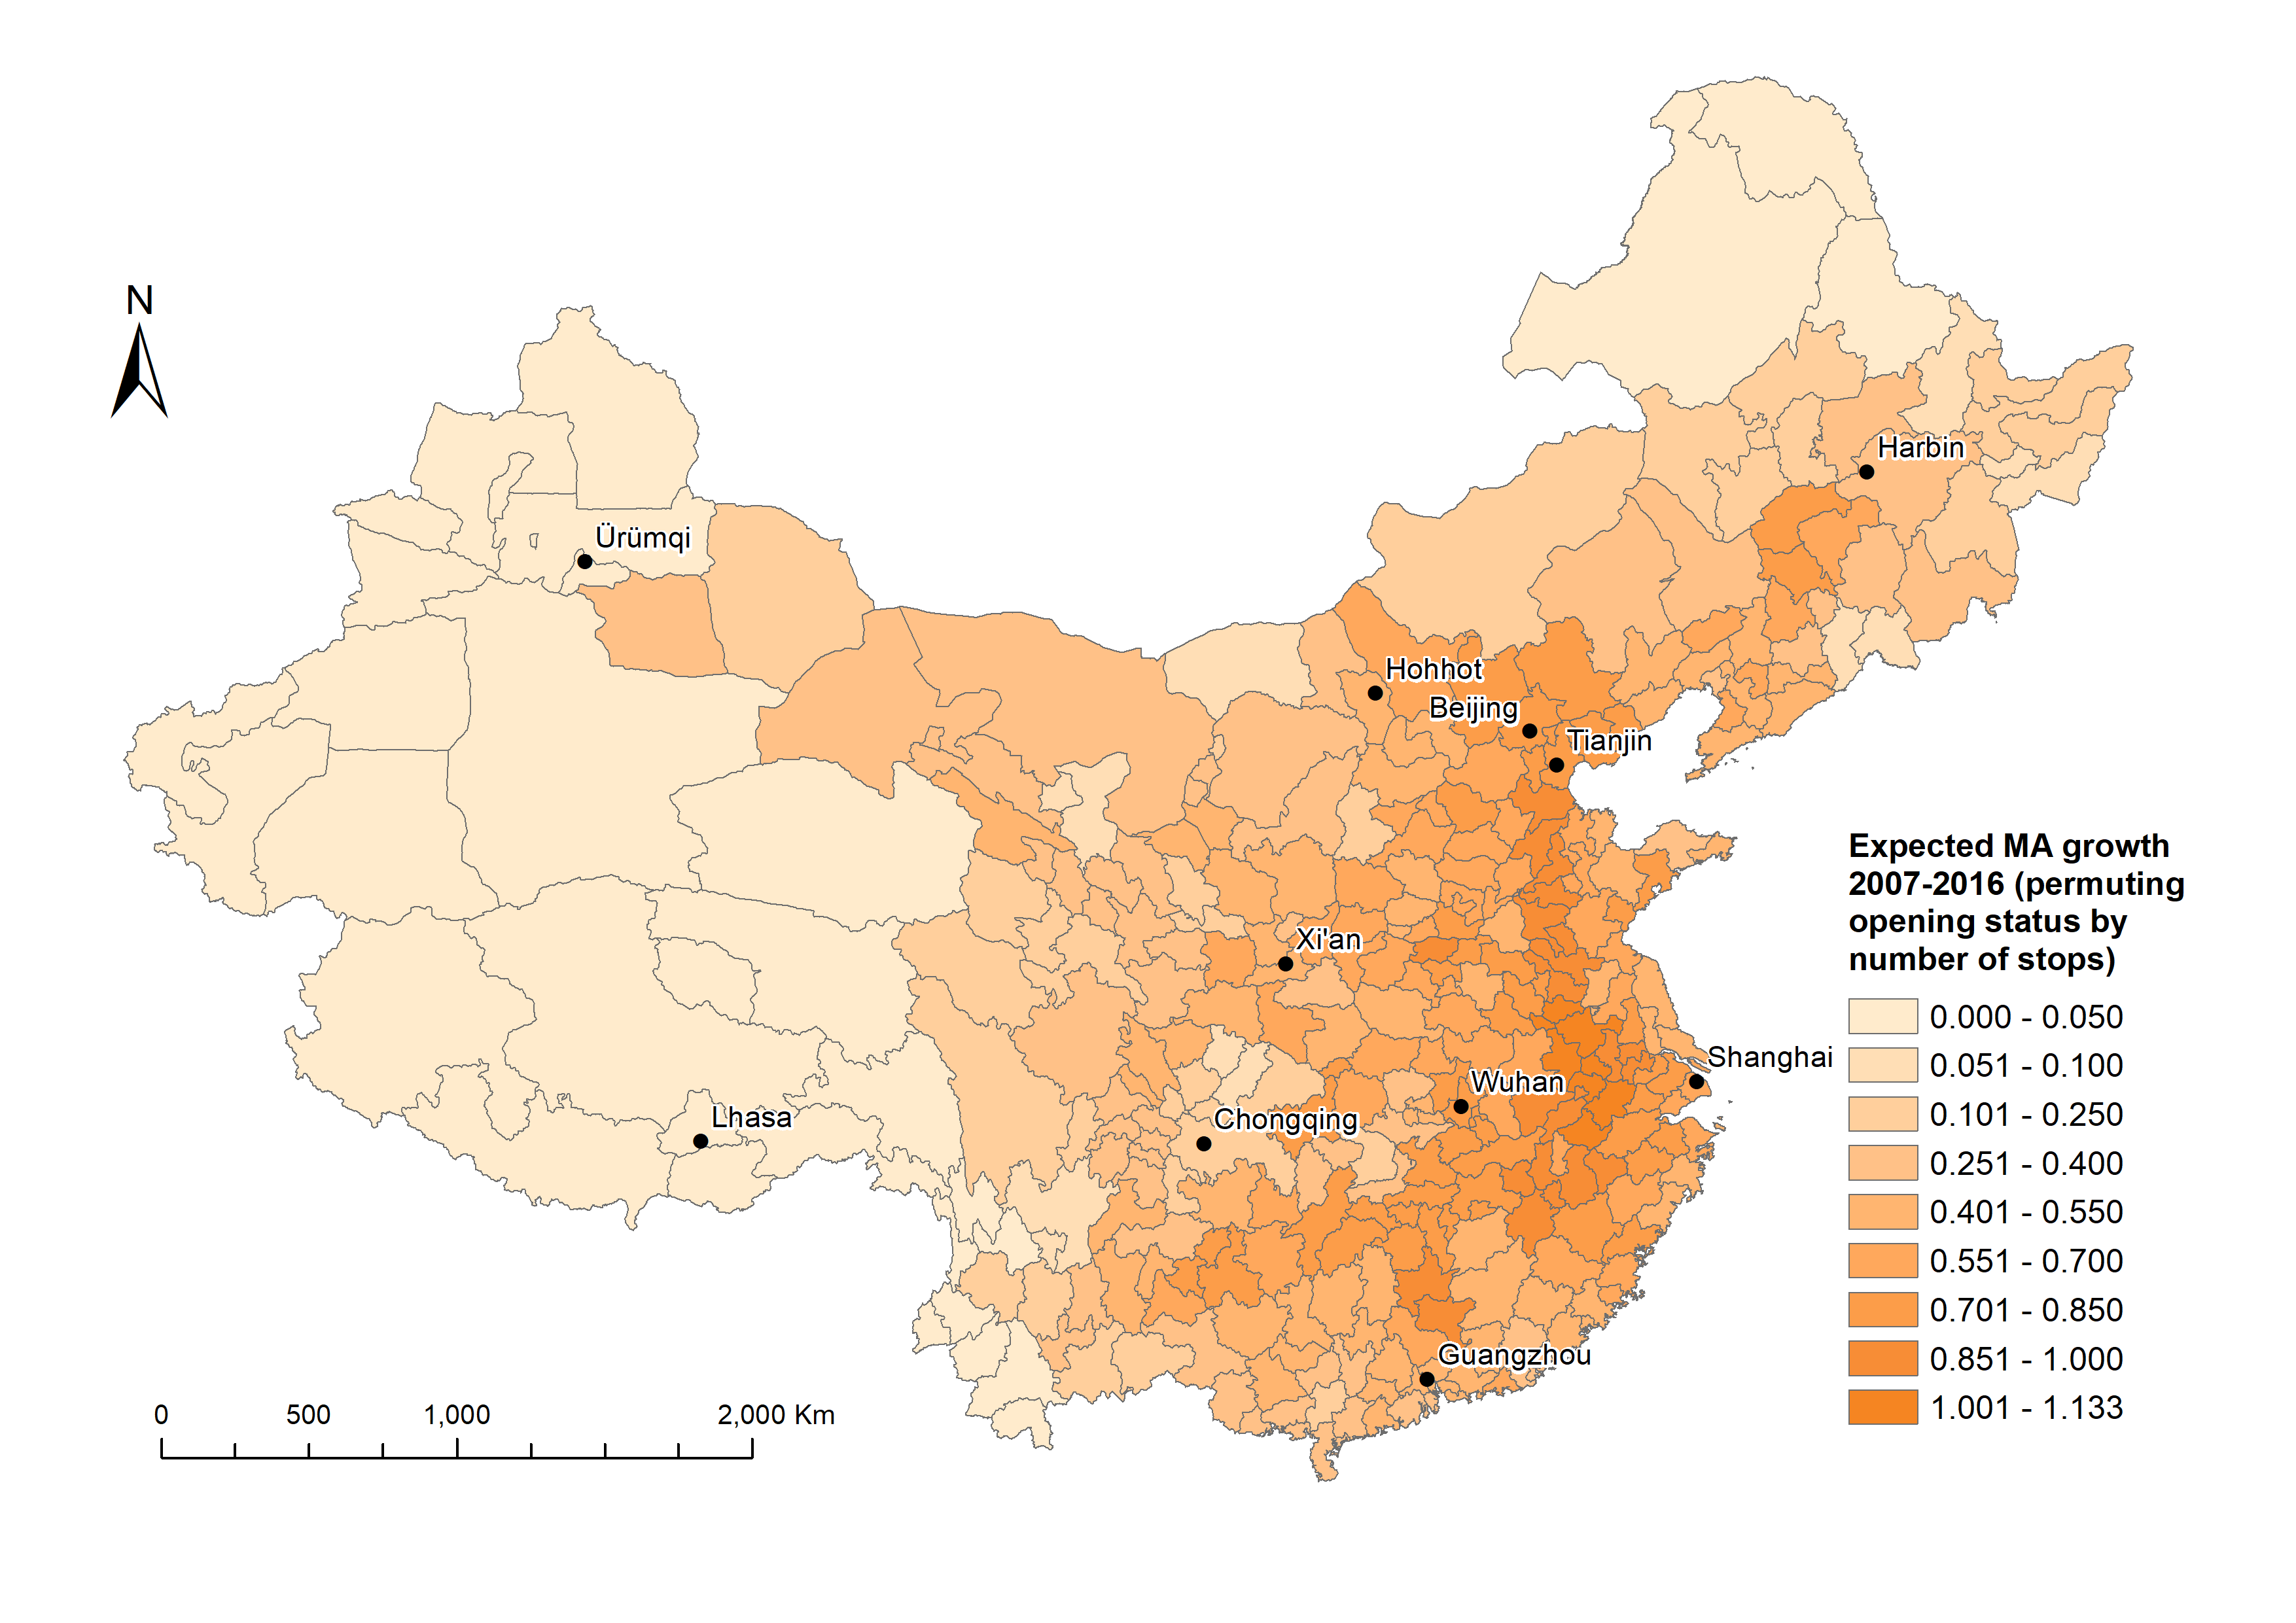
\includegraphics[trim={1cm 0.5cm 0cm 1cm},clip,width=11cm]{lecture_includes/NlinkExpected2016.png}
	
	\phantom{X}
	\end{center}
\end{frame}


\begin{frame}{Recentered Market Access Growth (2007--2016), $\tilde z_i$}
	\begin{center}
	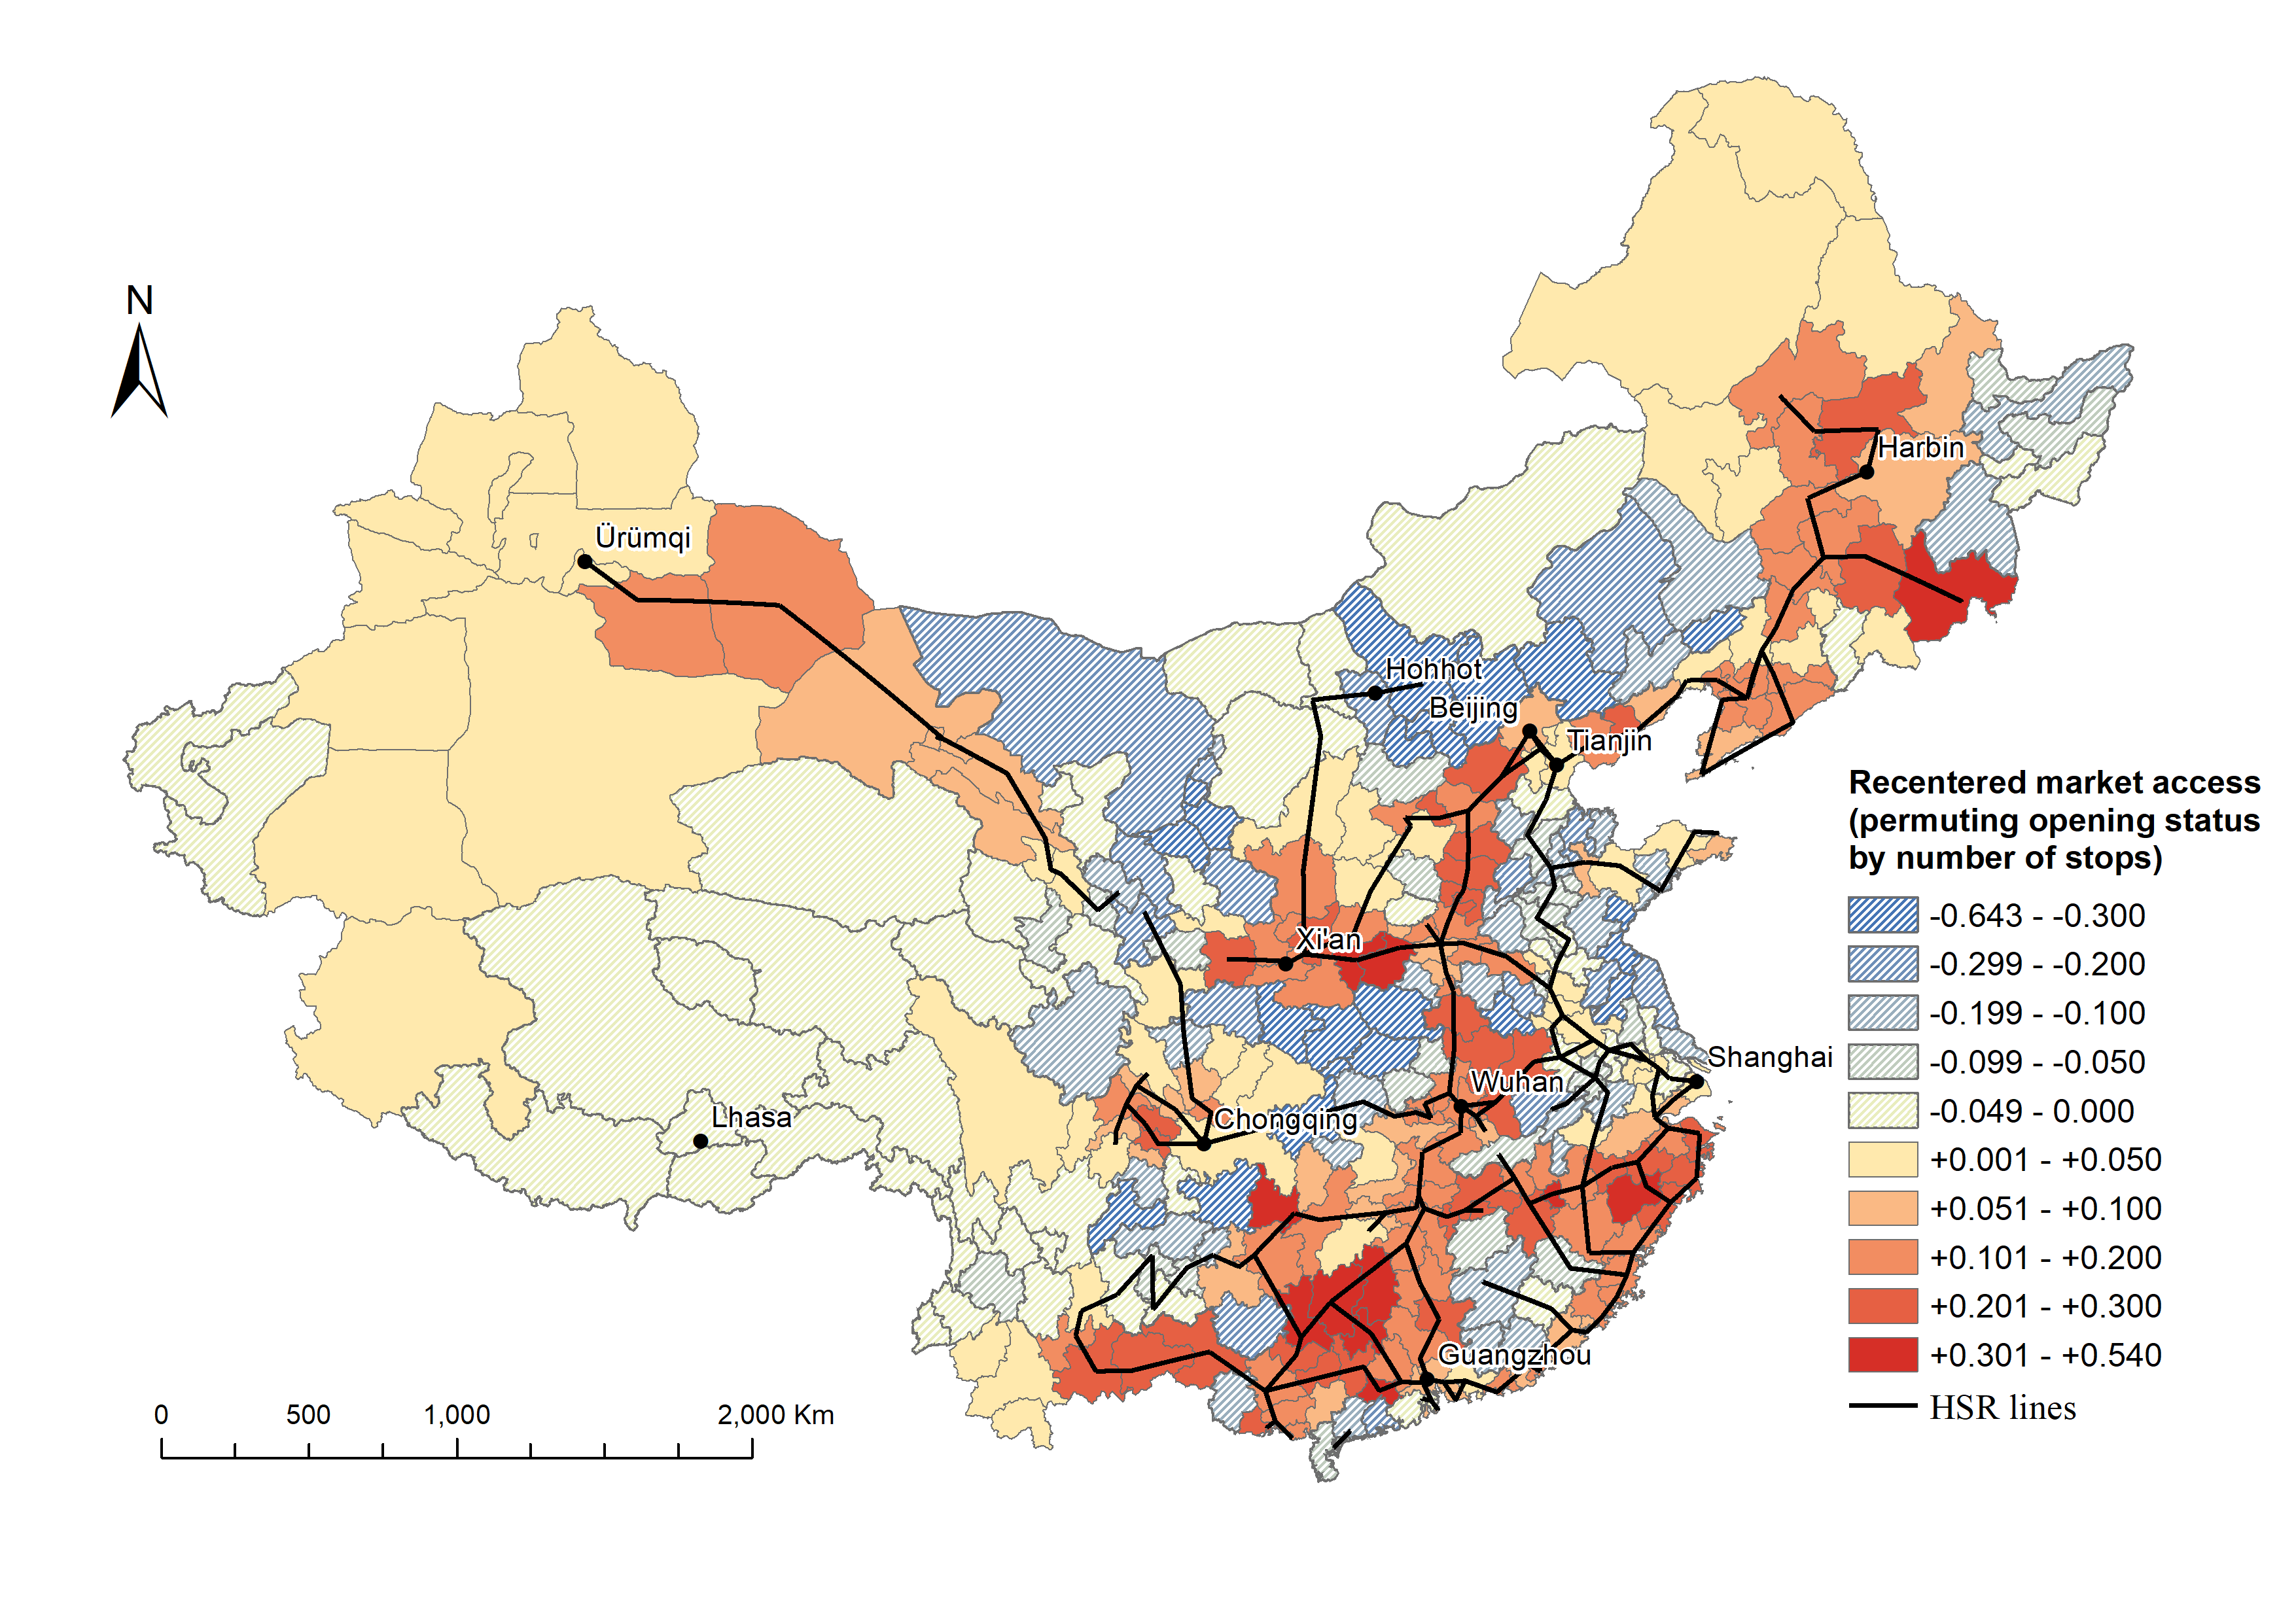
\includegraphics[trim={1cm 0.5cm 0cm 1cm},clip,width=11cm]{lecture_includes/NlinkRecentered2016.png}
	\end{center}
\end{frame}

\begin{frame}[label=HSRSpecTests]{Market Access Balance Regressions}
\begin{center}
\vspace{-0.4cm}
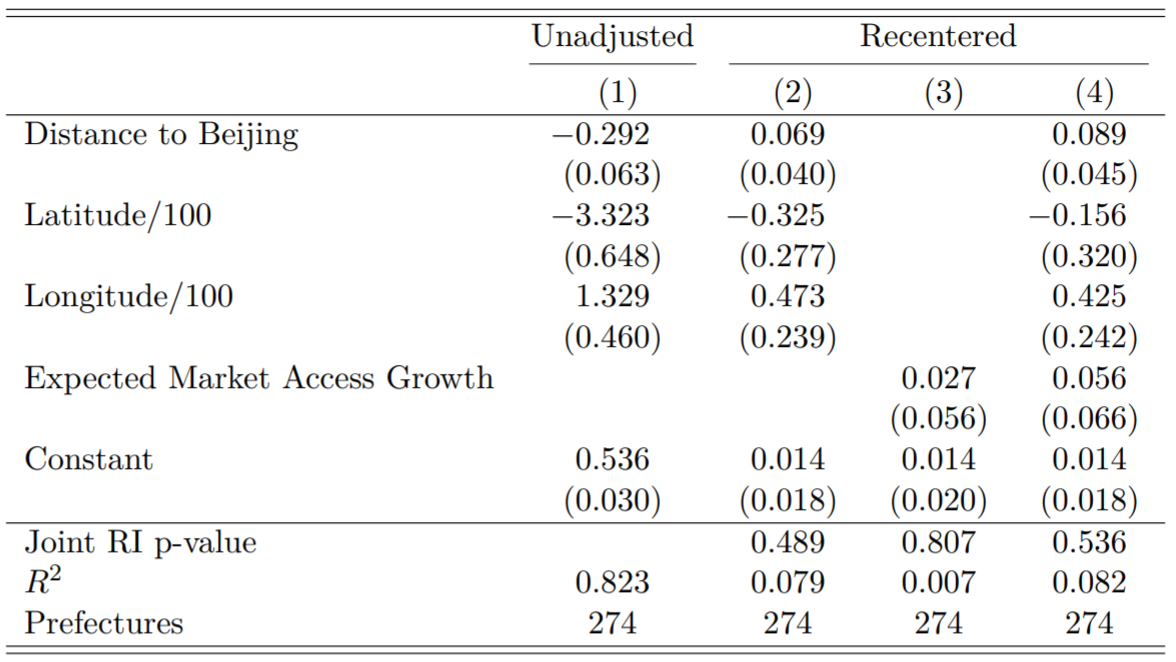
\includegraphics[width=12cm]{lecture_includes/spec_test.png}

\footnotesize{Regressions of unadjusted and recentered market access growth on geographic features. Spatial-clustered standard errors in parentheses.}

\end{center}

\end{frame}

\begin{frame}[label=HsrRcScatter]{Recentered MA Doesn't Predict Employment Growth!}
	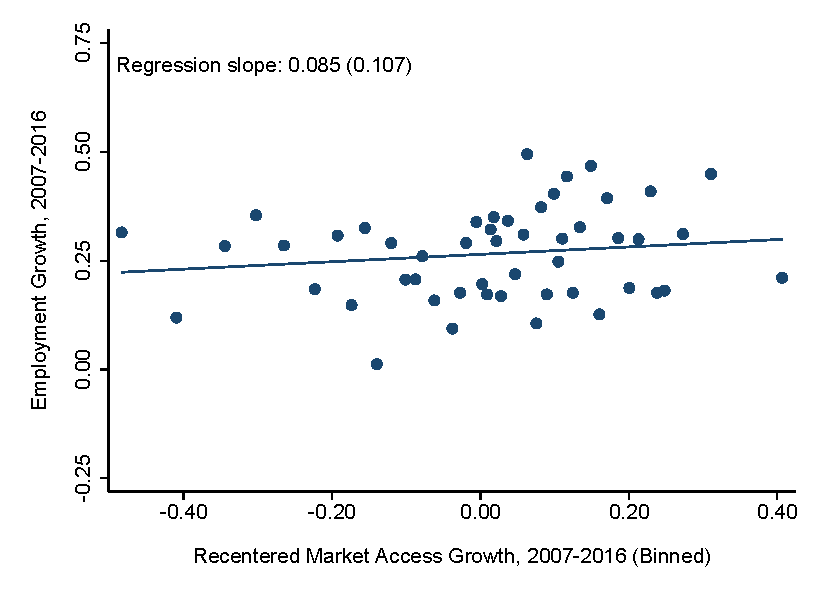
\includegraphics[width=\textwidth]{lecture_includes/emp_rc_nlink_binscatter.pdf} 
\end{frame}

\begin{frame}[label=HSRTable]{Adjusted Estimates of Market Access Effects}
	\begin{center}
	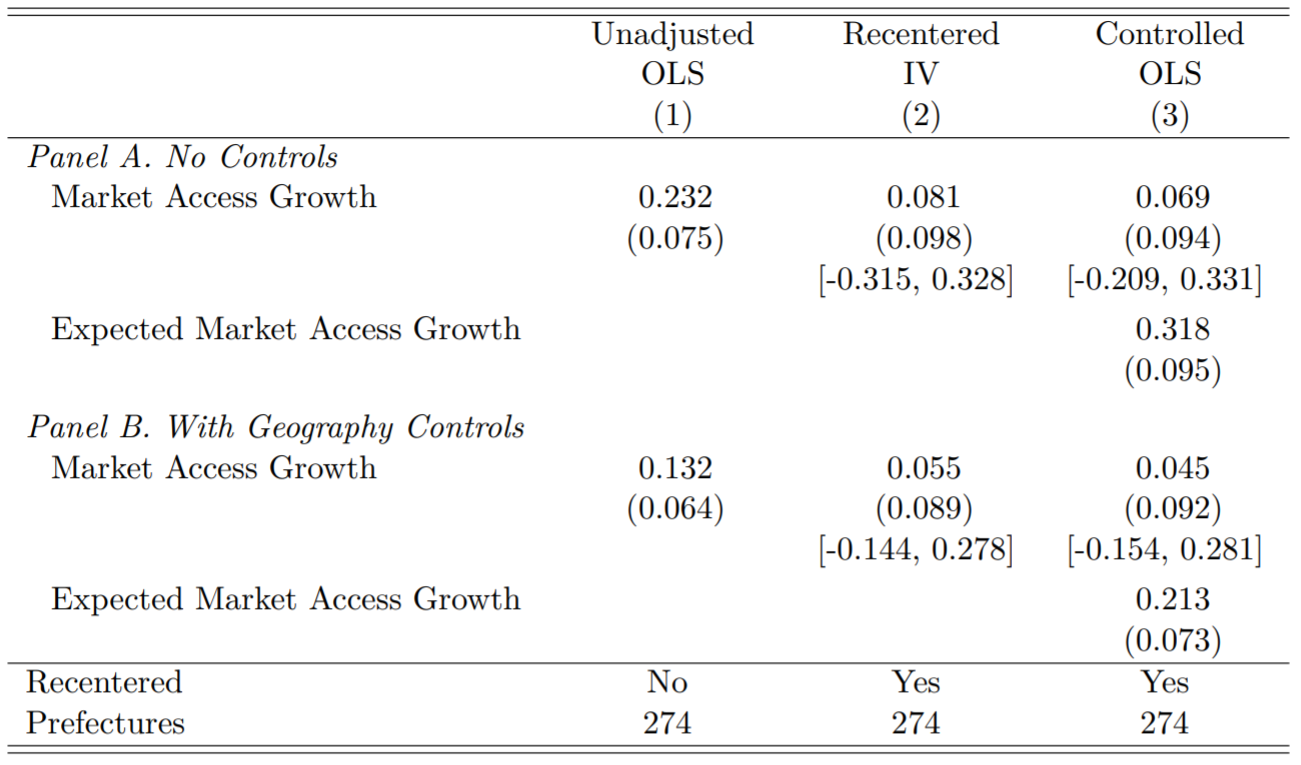
\includegraphics[width=0.9\textwidth]{lecture_includes/hsr_tab.png}
	
	\footnotesize{Regressions of log employment growth on log market access growth in 2007--2016. Spatial-clustered standard errors in parentheses; permutation-based 95\% CI in brackets}
	\end{center}
\end{frame}

\subsection{Medicaid Eligibility Effects}
\begin{frame}[label=ACA]{App. 2: Efficient Estimation of Medicaid Effects}
\vspace{-0.1cm}
\textbf{Setting}: U.S. Medicaid, partially expanded in 2014 under the ACA
\vspace{0.1cm}
	\begin{itemize}
	\item 19 of 43 states with low Medicaid coverage expanded to 138\% FPL
	\vspace{0.1cm}
	\item View \bgSun{expansion decisions} as random across states with same-party governors, but not \bgElectricViolet{household demographics} or \bgElectricViolet{pre-2014 policy}
	\vspace{0.1cm}
	\item Outcomes: Medicaid takeup and private insurance crowdout
\end{itemize}

\vspace{0.2cm}\pause
We compare two estimators, both valid under the same assumptions:
\begin{itemize}
	\vspace{0.1cm}
	\item Simulated IV: use state-level variation only (i.e. expansion dummy)
	\vspace{0.1cm}
	\item Recentered IV: predict eligibility from expansion decisions \& non-random demographics, and recenter
	\end{itemize}\pause{}
\vspace{0.2cm}
Via non-random variation, recentered IV has $\approx 3$ times smaller SEs
\end{frame}

\begin{frame}{Estimates with Simulated vs. Recentered IV}
	\begin{center}
	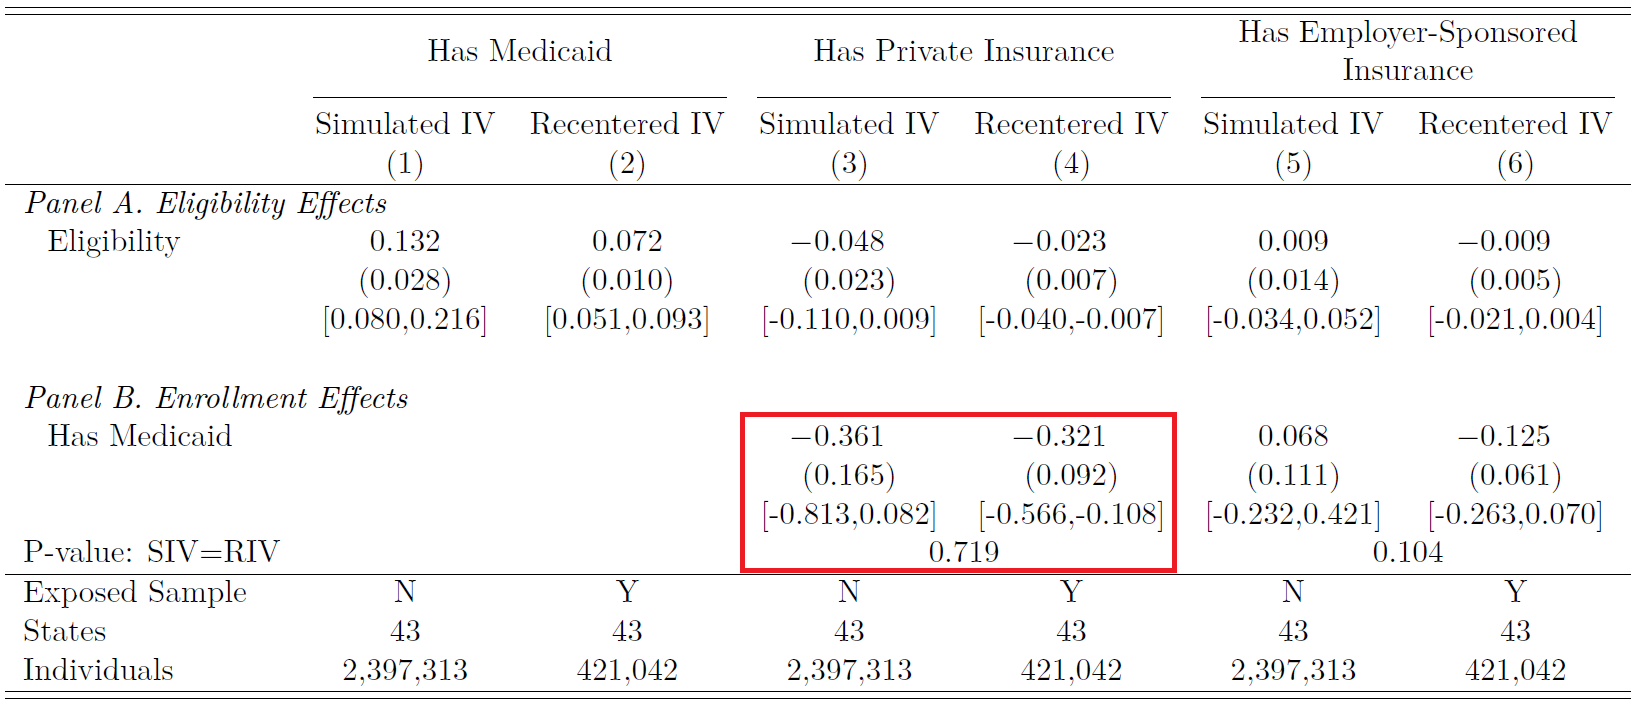
\includegraphics[width=1\textwidth]{lecture_includes/aca_ss.png}
	\end{center}

\footnotesize{1\% ACS sample of non-disabled adults in 2013--14, diff-in-diff IV regressions using one of the two instruments. Controls include state and year fixed effects and an indicator for Republican governor interacted with year. State-clustered standard errors in parentheses; wild score bootstrap 95\% CI in brackets} 
\end{frame}

\section{Concluding Thoughts}
\begin{frame}{Conclusions}
In both linear SSIV and more elaborate settings, the most important thing is to decide \emph{ex ante} what identifying variation you want to use\smallskip\pause{}
\begin{itemize}
\item When leveraging a natural experiment, recentering (e.g. controlling for sum-of-shares, in linear SSIV) can help\smallskip\pause{}
\item Non-experimental assumptions (e.g. parallel trends) typically require other approaches \smallskip
\item The source of variation can guide inference considerations
\end{itemize}\medskip\pause{}

After deciding + appropriately adjusting the analysis, try to falsify the identifying variation (\emph{ex post}) -- via balance or pre-trend tests\bigskip\pause{}

Much more work to be done on the various econometrics here!
\end{frame}


\begin{frame}{Keep Calm and SSIV On!}

\begin{center}
Good luck on your future adventures with SSIV!

\bigskip
\url{peter_hull@brown.edu}

\bigskip
 \url{@instrumenthull}
\end{center}
\end{frame}

\end{document}
